\documentclass[twoside]{book}

% Packages required by doxygen
\usepackage{fixltx2e}
\usepackage{calc}
\usepackage{doxygen}
\usepackage[export]{adjustbox} % also loads graphicx
\usepackage{graphicx}
\usepackage[utf8]{inputenc}
\usepackage{makeidx}
\usepackage{multicol}
\usepackage{multirow}
\PassOptionsToPackage{warn}{textcomp}
\usepackage{textcomp}
\usepackage[nointegrals]{wasysym}
\usepackage[table]{xcolor}

% Font selection
\usepackage[T1]{fontenc}
\usepackage[scaled=.90]{helvet}
\usepackage{courier}
\usepackage{amssymb}
\usepackage{sectsty}
\renewcommand{\familydefault}{\sfdefault}
\allsectionsfont{%
  \fontseries{bc}\selectfont%
  \color{darkgray}%
}
\renewcommand{\DoxyLabelFont}{%
  \fontseries{bc}\selectfont%
  \color{darkgray}%
}
\newcommand{\+}{\discretionary{\mbox{\scriptsize$\hookleftarrow$}}{}{}}

% Page & text layout
\usepackage{geometry}
\geometry{%
  a4paper,%
  top=2.5cm,%
  bottom=2.5cm,%
  left=2.5cm,%
  right=2.5cm%
}
\tolerance=750
\hfuzz=15pt
\hbadness=750
\setlength{\emergencystretch}{15pt}
\setlength{\parindent}{0cm}
\setlength{\parskip}{3ex plus 2ex minus 2ex}
\makeatletter
\renewcommand{\paragraph}{%
  \@startsection{paragraph}{4}{0ex}{-1.0ex}{1.0ex}{%
    \normalfont\normalsize\bfseries\SS@parafont%
  }%
}
\renewcommand{\subparagraph}{%
  \@startsection{subparagraph}{5}{0ex}{-1.0ex}{1.0ex}{%
    \normalfont\normalsize\bfseries\SS@subparafont%
  }%
}
\makeatother

% Headers & footers
\usepackage{fancyhdr}
\pagestyle{fancyplain}
\fancyhead[LE]{\fancyplain{}{\bfseries\thepage}}
\fancyhead[CE]{\fancyplain{}{}}
\fancyhead[RE]{\fancyplain{}{\bfseries\leftmark}}
\fancyhead[LO]{\fancyplain{}{\bfseries\rightmark}}
\fancyhead[CO]{\fancyplain{}{}}
\fancyhead[RO]{\fancyplain{}{\bfseries\thepage}}
\fancyfoot[LE]{\fancyplain{}{}}
\fancyfoot[CE]{\fancyplain{}{}}
\fancyfoot[RE]{\fancyplain{}{\bfseries\scriptsize Generated by Doxygen }}
\fancyfoot[LO]{\fancyplain{}{\bfseries\scriptsize Generated by Doxygen }}
\fancyfoot[CO]{\fancyplain{}{}}
\fancyfoot[RO]{\fancyplain{}{}}
\renewcommand{\footrulewidth}{0.4pt}
\renewcommand{\chaptermark}[1]{%
  \markboth{#1}{}%
}
\renewcommand{\sectionmark}[1]{%
  \markright{\thesection\ #1}%
}

% Indices & bibliography
\usepackage{natbib}
\usepackage[titles]{tocloft}
\setcounter{tocdepth}{3}
\setcounter{secnumdepth}{5}
\makeindex

% Hyperlinks (required, but should be loaded last)
\usepackage{ifpdf}
\ifpdf
  \usepackage[pdftex,pagebackref=true]{hyperref}
\else
  \usepackage[ps2pdf,pagebackref=true]{hyperref}
\fi
\hypersetup{%
  colorlinks=true,%
  linkcolor=blue,%
  citecolor=blue,%
  unicode%
}

% Custom commands
\newcommand{\clearemptydoublepage}{%
  \newpage{\pagestyle{empty}\cleardoublepage}%
}

\usepackage{caption}
\captionsetup{labelsep=space,justification=centering,font={bf},singlelinecheck=off,skip=4pt,position=top}

%===== C O N T E N T S =====

\begin{document}

% Titlepage & ToC
\hypersetup{pageanchor=false,
             bookmarksnumbered=true,
             pdfencoding=unicode
            }
\pagenumbering{alph}
\begin{titlepage}
\vspace*{7cm}
\begin{center}%
{\Large Ware\+House\+Manager }\\
\vspace*{1cm}
{\large Generated by Doxygen 1.8.14}\\
\end{center}
\end{titlepage}
\clearemptydoublepage
\pagenumbering{roman}
\tableofcontents
\clearemptydoublepage
\pagenumbering{arabic}
\hypersetup{pageanchor=true}

%--- Begin generated contents ---
\chapter{Hierarchical Index}
\section{Class Hierarchy}
This inheritance list is sorted roughly, but not completely, alphabetically\+:\begin{DoxyCompactList}
\item \contentsline{section}{Article}{\pageref{class_article}}{}
\item \contentsline{section}{Database}{\pageref{class_database}}{}
\item \contentsline{section}{Emballage}{\pageref{class_emballage}}{}
\item \contentsline{section}{Fournisseur}{\pageref{class_fournisseur}}{}
\item \contentsline{section}{Livraison}{\pageref{class_livraison}}{}
\item Q\+Dialog\begin{DoxyCompactList}
\item \contentsline{section}{Login}{\pageref{class_login}}{}
\end{DoxyCompactList}
\item Q\+Main\+Window\begin{DoxyCompactList}
\item \contentsline{section}{Main\+Window}{\pageref{class_main_window}}{}
\end{DoxyCompactList}
\item \contentsline{section}{Utilisateur}{\pageref{class_utilisateur}}{}
\end{DoxyCompactList}

\chapter{Class Index}
\section{Class List}
Here are the classes, structs, unions and interfaces with brief descriptions\+:\begin{DoxyCompactList}
\item\contentsline{section}{\mbox{\hyperlink{class_article}{Article}} \\*Classe \mbox{\hyperlink{class_article}{Article}} permettant de gerer les articles }{\pageref{class_article}}{}
\item\contentsline{section}{\mbox{\hyperlink{class_database}{Database}} }{\pageref{class_database}}{}
\item\contentsline{section}{\mbox{\hyperlink{class_emballage}{Emballage}} \\*Classe emballage permettant de gerer les emballages }{\pageref{class_emballage}}{}
\item\contentsline{section}{\mbox{\hyperlink{class_fenetre_login}{Fenetre\+Login}} }{\pageref{class_fenetre_login}}{}
\item\contentsline{section}{\mbox{\hyperlink{class_fournisseur}{Fournisseur}} }{\pageref{class_fournisseur}}{}
\item\contentsline{section}{\mbox{\hyperlink{class_livraison}{Livraison}} }{\pageref{class_livraison}}{}
\item\contentsline{section}{\mbox{\hyperlink{class_login}{Login}} }{\pageref{class_login}}{}
\item\contentsline{section}{\mbox{\hyperlink{class_main_window}{Main\+Window}} }{\pageref{class_main_window}}{}
\item\contentsline{section}{\mbox{\hyperlink{classmenuwindow}{menuwindow}} }{\pageref{classmenuwindow}}{}
\item\contentsline{section}{\mbox{\hyperlink{class_utilisateur}{Utilisateur}} \\*Classe \mbox{\hyperlink{class_utilisateur}{Utilisateur}} permettant de gerer les utilisateurs }{\pageref{class_utilisateur}}{}
\end{DoxyCompactList}

\chapter{File Index}
\section{File List}
Here is a list of all documented files with brief descriptions\+:\begin{DoxyCompactList}
\item\contentsline{section}{C\+:/\+Users/adai01/\+Desktop/\+Ware\+House\+Manager/\mbox{\hyperlink{article_8h}{article.\+h}} \\*Gestion des articles }{\pageref{article_8h}}{}
\item\contentsline{section}{C\+:/\+Users/adai01/\+Desktop/\+Ware\+House\+Manager/\mbox{\hyperlink{database_8h}{database.\+h}} \\*Gestion de toutes les requetes S\+QL }{\pageref{database_8h}}{}
\item\contentsline{section}{C\+:/\+Users/adai01/\+Desktop/\+Ware\+House\+Manager/\mbox{\hyperlink{emballage_8h}{emballage.\+h}} \\*Gestion des emballages }{\pageref{emballage_8h}}{}
\item\contentsline{section}{C\+:/\+Users/adai01/\+Desktop/\+Ware\+House\+Manager/\mbox{\hyperlink{fournisseur_8h}{fournisseur.\+h}} \\*Gestion des fournisseurs }{\pageref{fournisseur_8h}}{}
\item\contentsline{section}{C\+:/\+Users/adai01/\+Desktop/\+Ware\+House\+Manager/\mbox{\hyperlink{livraison_8h}{livraison.\+h}} \\*Gestion des livraisons }{\pageref{livraison_8h}}{}
\item\contentsline{section}{C\+:/\+Users/adai01/\+Desktop/\+Ware\+House\+Manager/\mbox{\hyperlink{login_8h}{login.\+h}} \\*Gestion des logins }{\pageref{login_8h}}{}
\item\contentsline{section}{C\+:/\+Users/adai01/\+Desktop/\+Ware\+House\+Manager/\mbox{\hyperlink{mainwindow_8h}{mainwindow.\+h}} \\*Fenetre principale de l\textquotesingle{}application }{\pageref{mainwindow_8h}}{}
\item\contentsline{section}{C\+:/\+Users/adai01/\+Desktop/\+Ware\+House\+Manager/\mbox{\hyperlink{utilisateur_8h}{utilisateur.\+h}} \\*Gestion des utilisateurs }{\pageref{utilisateur_8h}}{}
\end{DoxyCompactList}

\chapter{Class Documentation}
\hypertarget{class_article}{}\section{Article Class Reference}
\label{class_article}\index{Article@{Article}}


Classe \mbox{\hyperlink{class_article}{Article}} permettant de gerer les articles.  




{\ttfamily \#include $<$article.\+h$>$}

\subsection*{Public Member Functions}
\begin{DoxyCompactItemize}
\item 
\mbox{\hyperlink{class_article_aba1b3142ede0565d468cb4135384c96f}{Article}} ()
\begin{DoxyCompactList}\small\item\em \mbox{\hyperlink{class_article}{Article}} Constructeur vide de la classe article. \end{DoxyCompactList}\item 
\mbox{\hyperlink{class_article_a7422cbd424c70f209ef1bf83ea0fd42e}{Article}} (Q\+String \mbox{\hyperlink{class_article_a302186fb47a2b9bd8736bab99fe3ec75}{code\+Article}}, Q\+String \mbox{\hyperlink{class_article_a120a68e558a25bfd50bcc0ace22d6eef}{designation\+Article}}, int \mbox{\hyperlink{class_article_aaf339d5933ee1e8386dd57a8f84a9602}{poids\+Article}}, Q\+String \mbox{\hyperlink{class_article_a97f4fcb1534dbe969fcb2f6f2a8fdbd7}{emplacement\+Article}}, Q\+String \mbox{\hyperlink{class_article_a9ee6bb591aaba7535eac3d5965467965}{emballage\+Article}})
\begin{DoxyCompactList}\small\item\em \mbox{\hyperlink{class_article}{Article}} Constructeur permettant de construire un objet article avec les paramètres. \end{DoxyCompactList}\item 
Q\+String \mbox{\hyperlink{class_article_aa7a4dfd88216d2cea5d2393fac2af585}{Get\+Code\+Article}} ()
\begin{DoxyCompactList}\small\item\em Get\+Code\+Article. \end{DoxyCompactList}\item 
Q\+String \mbox{\hyperlink{class_article_af9b0da3a793b4a0dcfe8e97b24ac4f79}{Get\+Designation\+Article}} ()
\begin{DoxyCompactList}\small\item\em Get\+Designation\+Article. \end{DoxyCompactList}\item 
int \mbox{\hyperlink{class_article_a0509109984e6d86e783c457ce70d13a7}{Get\+Poids\+Article}} ()
\begin{DoxyCompactList}\small\item\em Get\+Poids\+Article. \end{DoxyCompactList}\item 
Q\+String \mbox{\hyperlink{class_article_aca48728ecc7862026b40b18db12591fa}{Get\+Emplacement\+Article}} ()
\begin{DoxyCompactList}\small\item\em Get\+Emplacement\+Article. \end{DoxyCompactList}\item 
Q\+String \mbox{\hyperlink{class_article_aa086c1a1aa8af81fb34c9a20b05d0155}{Get\+Emballage\+Article}} ()
\begin{DoxyCompactList}\small\item\em Get\+Emballage\+Article. \end{DoxyCompactList}\item 
void \mbox{\hyperlink{class_article_a5300f5a6247dd931cb411d7ff1721d7f}{Set\+Code\+Article}} (Q\+String \mbox{\hyperlink{class_article_a302186fb47a2b9bd8736bab99fe3ec75}{code\+Article}})
\begin{DoxyCompactList}\small\item\em Set\+Code\+Article. \end{DoxyCompactList}\item 
void \mbox{\hyperlink{class_article_a6ee68c7584a20323039ab5065c34eb81}{Set\+Designation\+Article}} (Q\+String \mbox{\hyperlink{class_article_a120a68e558a25bfd50bcc0ace22d6eef}{designation\+Article}})
\begin{DoxyCompactList}\small\item\em Set\+Designation\+Article. \end{DoxyCompactList}\item 
void \mbox{\hyperlink{class_article_af2412d92eb7d53ca7566755a900653c0}{Set\+Poids\+Article}} (int \mbox{\hyperlink{class_article_aaf339d5933ee1e8386dd57a8f84a9602}{poids\+Article}})
\begin{DoxyCompactList}\small\item\em Set\+Poids\+Article. \end{DoxyCompactList}\item 
void \mbox{\hyperlink{class_article_ae543837747d1022bd91afb5ca7e7cc32}{Set\+Emplacement\+Article}} (Q\+String \mbox{\hyperlink{class_article_a97f4fcb1534dbe969fcb2f6f2a8fdbd7}{emplacement\+Article}})
\begin{DoxyCompactList}\small\item\em Set\+Emplacement\+Article. \end{DoxyCompactList}\item 
void \mbox{\hyperlink{class_article_abfde880e0537319807827026d0d7897f}{Set\+Emballage\+Article}} (Q\+String \mbox{\hyperlink{class_article_a9ee6bb591aaba7535eac3d5965467965}{emballage\+Article}})
\begin{DoxyCompactList}\small\item\em Set\+Emballage\+Article. \end{DoxyCompactList}\end{DoxyCompactItemize}
\subsection*{Private Attributes}
\begin{DoxyCompactItemize}
\item 
\mbox{\Hypertarget{class_article_a302186fb47a2b9bd8736bab99fe3ec75}\label{class_article_a302186fb47a2b9bd8736bab99fe3ec75}} 
Q\+String \mbox{\hyperlink{class_article_a302186fb47a2b9bd8736bab99fe3ec75}{code\+Article}}
\begin{DoxyCompactList}\small\item\em code\+Article \end{DoxyCompactList}\item 
\mbox{\Hypertarget{class_article_a120a68e558a25bfd50bcc0ace22d6eef}\label{class_article_a120a68e558a25bfd50bcc0ace22d6eef}} 
Q\+String \mbox{\hyperlink{class_article_a120a68e558a25bfd50bcc0ace22d6eef}{designation\+Article}}
\begin{DoxyCompactList}\small\item\em designation\+Article \end{DoxyCompactList}\item 
\mbox{\Hypertarget{class_article_aaf339d5933ee1e8386dd57a8f84a9602}\label{class_article_aaf339d5933ee1e8386dd57a8f84a9602}} 
int \mbox{\hyperlink{class_article_aaf339d5933ee1e8386dd57a8f84a9602}{poids\+Article}}
\begin{DoxyCompactList}\small\item\em poids\+Article \end{DoxyCompactList}\item 
\mbox{\Hypertarget{class_article_a97f4fcb1534dbe969fcb2f6f2a8fdbd7}\label{class_article_a97f4fcb1534dbe969fcb2f6f2a8fdbd7}} 
Q\+String \mbox{\hyperlink{class_article_a97f4fcb1534dbe969fcb2f6f2a8fdbd7}{emplacement\+Article}}
\begin{DoxyCompactList}\small\item\em emplacement\+Article \end{DoxyCompactList}\item 
\mbox{\Hypertarget{class_article_a9ee6bb591aaba7535eac3d5965467965}\label{class_article_a9ee6bb591aaba7535eac3d5965467965}} 
Q\+String \mbox{\hyperlink{class_article_a9ee6bb591aaba7535eac3d5965467965}{emballage\+Article}}
\begin{DoxyCompactList}\small\item\em emballage\+Article \end{DoxyCompactList}\end{DoxyCompactItemize}


\subsection{Detailed Description}
Classe \mbox{\hyperlink{class_article}{Article}} permettant de gerer les articles. 

\subsection{Constructor \& Destructor Documentation}
\mbox{\Hypertarget{class_article_aba1b3142ede0565d468cb4135384c96f}\label{class_article_aba1b3142ede0565d468cb4135384c96f}} 
\index{Article@{Article}!Article@{Article}}
\index{Article@{Article}!Article@{Article}}
\subsubsection{\texorpdfstring{Article()}{Article()}\hspace{0.1cm}{\footnotesize\ttfamily [1/2]}}
{\footnotesize\ttfamily Article\+::\+Article (\begin{DoxyParamCaption}{ }\end{DoxyParamCaption})}



\mbox{\hyperlink{class_article}{Article}} Constructeur vide de la classe article. 

\mbox{\hyperlink{class_article_aba1b3142ede0565d468cb4135384c96f}{Article\+::\+Article}}. \mbox{\Hypertarget{class_article_a7422cbd424c70f209ef1bf83ea0fd42e}\label{class_article_a7422cbd424c70f209ef1bf83ea0fd42e}} 
\index{Article@{Article}!Article@{Article}}
\index{Article@{Article}!Article@{Article}}
\subsubsection{\texorpdfstring{Article()}{Article()}\hspace{0.1cm}{\footnotesize\ttfamily [2/2]}}
{\footnotesize\ttfamily Article\+::\+Article (\begin{DoxyParamCaption}\item[{Q\+String}]{code\+Article,  }\item[{Q\+String}]{designation\+Article,  }\item[{int}]{poids\+Article,  }\item[{Q\+String}]{emplacement\+Article,  }\item[{Q\+String}]{emballage\+Article }\end{DoxyParamCaption})}



\mbox{\hyperlink{class_article}{Article}} Constructeur permettant de construire un objet article avec les paramètres. 

\mbox{\hyperlink{class_article_aba1b3142ede0565d468cb4135384c96f}{Article\+::\+Article}}.


\begin{DoxyParams}{Parameters}
{\em code\+Article} & \\
\hline
{\em designation\+Article} & \\
\hline
{\em poids\+Article} & \\
\hline
{\em emplacement\+Article} & \\
\hline
{\em emballage\+Article} & \\
\hline
\end{DoxyParams}


\subsection{Member Function Documentation}
\mbox{\Hypertarget{class_article_aa7a4dfd88216d2cea5d2393fac2af585}\label{class_article_aa7a4dfd88216d2cea5d2393fac2af585}} 
\index{Article@{Article}!Get\+Code\+Article@{Get\+Code\+Article}}
\index{Get\+Code\+Article@{Get\+Code\+Article}!Article@{Article}}
\subsubsection{\texorpdfstring{Get\+Code\+Article()}{GetCodeArticle()}}
{\footnotesize\ttfamily Q\+String Article\+::\+Get\+Code\+Article (\begin{DoxyParamCaption}{ }\end{DoxyParamCaption})}



Get\+Code\+Article. 

\mbox{\hyperlink{class_article_aa7a4dfd88216d2cea5d2393fac2af585}{Article\+::\+Get\+Code\+Article}}.

\begin{DoxyReturn}{Returns}
Retourne le code article (Q\+String)


\end{DoxyReturn}
\mbox{\Hypertarget{class_article_af9b0da3a793b4a0dcfe8e97b24ac4f79}\label{class_article_af9b0da3a793b4a0dcfe8e97b24ac4f79}} 
\index{Article@{Article}!Get\+Designation\+Article@{Get\+Designation\+Article}}
\index{Get\+Designation\+Article@{Get\+Designation\+Article}!Article@{Article}}
\subsubsection{\texorpdfstring{Get\+Designation\+Article()}{GetDesignationArticle()}}
{\footnotesize\ttfamily Q\+String Article\+::\+Get\+Designation\+Article (\begin{DoxyParamCaption}{ }\end{DoxyParamCaption})}



Get\+Designation\+Article. 

\mbox{\hyperlink{class_article_af9b0da3a793b4a0dcfe8e97b24ac4f79}{Article\+::\+Get\+Designation\+Article}}.

\begin{DoxyReturn}{Returns}
Retourne la designation de l\textquotesingle{}article (Q\+String)


\end{DoxyReturn}
\mbox{\Hypertarget{class_article_aa086c1a1aa8af81fb34c9a20b05d0155}\label{class_article_aa086c1a1aa8af81fb34c9a20b05d0155}} 
\index{Article@{Article}!Get\+Emballage\+Article@{Get\+Emballage\+Article}}
\index{Get\+Emballage\+Article@{Get\+Emballage\+Article}!Article@{Article}}
\subsubsection{\texorpdfstring{Get\+Emballage\+Article()}{GetEmballageArticle()}}
{\footnotesize\ttfamily Q\+String Article\+::\+Get\+Emballage\+Article (\begin{DoxyParamCaption}{ }\end{DoxyParamCaption})}



Get\+Emballage\+Article. 

\mbox{\hyperlink{class_article_aa086c1a1aa8af81fb34c9a20b05d0155}{Article\+::\+Get\+Emballage\+Article}}.

\begin{DoxyReturn}{Returns}
Retourne les dimensions de l\textquotesingle{}emballage (Q\+String)


\end{DoxyReturn}
\mbox{\Hypertarget{class_article_aca48728ecc7862026b40b18db12591fa}\label{class_article_aca48728ecc7862026b40b18db12591fa}} 
\index{Article@{Article}!Get\+Emplacement\+Article@{Get\+Emplacement\+Article}}
\index{Get\+Emplacement\+Article@{Get\+Emplacement\+Article}!Article@{Article}}
\subsubsection{\texorpdfstring{Get\+Emplacement\+Article()}{GetEmplacementArticle()}}
{\footnotesize\ttfamily Q\+String Article\+::\+Get\+Emplacement\+Article (\begin{DoxyParamCaption}{ }\end{DoxyParamCaption})}



Get\+Emplacement\+Article. 

\mbox{\hyperlink{class_article_aca48728ecc7862026b40b18db12591fa}{Article\+::\+Get\+Emplacement\+Article}}.

\begin{DoxyReturn}{Returns}
Retourne l\textquotesingle{}emplacement de l\textquotesingle{}article (Q\+String)


\end{DoxyReturn}
\mbox{\Hypertarget{class_article_a0509109984e6d86e783c457ce70d13a7}\label{class_article_a0509109984e6d86e783c457ce70d13a7}} 
\index{Article@{Article}!Get\+Poids\+Article@{Get\+Poids\+Article}}
\index{Get\+Poids\+Article@{Get\+Poids\+Article}!Article@{Article}}
\subsubsection{\texorpdfstring{Get\+Poids\+Article()}{GetPoidsArticle()}}
{\footnotesize\ttfamily int Article\+::\+Get\+Poids\+Article (\begin{DoxyParamCaption}{ }\end{DoxyParamCaption})}



Get\+Poids\+Article. 

\mbox{\hyperlink{class_article_a0509109984e6d86e783c457ce70d13a7}{Article\+::\+Get\+Poids\+Article}}.

\begin{DoxyReturn}{Returns}
Retourne le poids de l\textquotesingle{}artciel (Int)


\end{DoxyReturn}
\mbox{\Hypertarget{class_article_a5300f5a6247dd931cb411d7ff1721d7f}\label{class_article_a5300f5a6247dd931cb411d7ff1721d7f}} 
\index{Article@{Article}!Set\+Code\+Article@{Set\+Code\+Article}}
\index{Set\+Code\+Article@{Set\+Code\+Article}!Article@{Article}}
\subsubsection{\texorpdfstring{Set\+Code\+Article()}{SetCodeArticle()}}
{\footnotesize\ttfamily void Article\+::\+Set\+Code\+Article (\begin{DoxyParamCaption}\item[{Q\+String}]{code\+Article }\end{DoxyParamCaption})}



Set\+Code\+Article. 

\mbox{\hyperlink{class_article_a5300f5a6247dd931cb411d7ff1721d7f}{Article\+::\+Set\+Code\+Article}}.


\begin{DoxyParams}{Parameters}
{\em code\+Article} & \\
\hline
\end{DoxyParams}
\mbox{\Hypertarget{class_article_a6ee68c7584a20323039ab5065c34eb81}\label{class_article_a6ee68c7584a20323039ab5065c34eb81}} 
\index{Article@{Article}!Set\+Designation\+Article@{Set\+Designation\+Article}}
\index{Set\+Designation\+Article@{Set\+Designation\+Article}!Article@{Article}}
\subsubsection{\texorpdfstring{Set\+Designation\+Article()}{SetDesignationArticle()}}
{\footnotesize\ttfamily void Article\+::\+Set\+Designation\+Article (\begin{DoxyParamCaption}\item[{Q\+String}]{designation\+Article }\end{DoxyParamCaption})}



Set\+Designation\+Article. 

\mbox{\hyperlink{class_article_a6ee68c7584a20323039ab5065c34eb81}{Article\+::\+Set\+Designation\+Article}}.


\begin{DoxyParams}{Parameters}
{\em designation\+Article} & \\
\hline
\end{DoxyParams}
\mbox{\Hypertarget{class_article_abfde880e0537319807827026d0d7897f}\label{class_article_abfde880e0537319807827026d0d7897f}} 
\index{Article@{Article}!Set\+Emballage\+Article@{Set\+Emballage\+Article}}
\index{Set\+Emballage\+Article@{Set\+Emballage\+Article}!Article@{Article}}
\subsubsection{\texorpdfstring{Set\+Emballage\+Article()}{SetEmballageArticle()}}
{\footnotesize\ttfamily void Article\+::\+Set\+Emballage\+Article (\begin{DoxyParamCaption}\item[{Q\+String}]{emballage\+Article }\end{DoxyParamCaption})}



Set\+Emballage\+Article. 

\mbox{\hyperlink{class_article_abfde880e0537319807827026d0d7897f}{Article\+::\+Set\+Emballage\+Article}}.


\begin{DoxyParams}{Parameters}
{\em emballage\+Article} & \\
\hline
\end{DoxyParams}
\mbox{\Hypertarget{class_article_ae543837747d1022bd91afb5ca7e7cc32}\label{class_article_ae543837747d1022bd91afb5ca7e7cc32}} 
\index{Article@{Article}!Set\+Emplacement\+Article@{Set\+Emplacement\+Article}}
\index{Set\+Emplacement\+Article@{Set\+Emplacement\+Article}!Article@{Article}}
\subsubsection{\texorpdfstring{Set\+Emplacement\+Article()}{SetEmplacementArticle()}}
{\footnotesize\ttfamily void Article\+::\+Set\+Emplacement\+Article (\begin{DoxyParamCaption}\item[{Q\+String}]{emplacement\+Article }\end{DoxyParamCaption})}



Set\+Emplacement\+Article. 

\mbox{\hyperlink{class_article_ae543837747d1022bd91afb5ca7e7cc32}{Article\+::\+Set\+Emplacement\+Article}}.


\begin{DoxyParams}{Parameters}
{\em emplacement\+Article} & \\
\hline
\end{DoxyParams}
\mbox{\Hypertarget{class_article_af2412d92eb7d53ca7566755a900653c0}\label{class_article_af2412d92eb7d53ca7566755a900653c0}} 
\index{Article@{Article}!Set\+Poids\+Article@{Set\+Poids\+Article}}
\index{Set\+Poids\+Article@{Set\+Poids\+Article}!Article@{Article}}
\subsubsection{\texorpdfstring{Set\+Poids\+Article()}{SetPoidsArticle()}}
{\footnotesize\ttfamily void Article\+::\+Set\+Poids\+Article (\begin{DoxyParamCaption}\item[{int}]{poids\+Article }\end{DoxyParamCaption})}



Set\+Poids\+Article. 

\mbox{\hyperlink{class_article_af2412d92eb7d53ca7566755a900653c0}{Article\+::\+Set\+Poids\+Article}}.


\begin{DoxyParams}{Parameters}
{\em poids\+Article} & \\
\hline
\end{DoxyParams}


The documentation for this class was generated from the following files\+:\begin{DoxyCompactItemize}
\item 
C\+:/\+Users/adai01/\+Desktop/\+Ware\+House\+Manager/\mbox{\hyperlink{article_8h}{article.\+h}}\item 
C\+:/\+Users/adai01/\+Desktop/\+Ware\+House\+Manager/article.\+cpp\end{DoxyCompactItemize}

\hypertarget{class_database}{}\section{Database Class Reference}
\label{class_database}\index{Database@{Database}}


Classe \mbox{\hyperlink{class_database}{Database}} permettant de gerer les requetes S\+QL. Dans cette classe toutes les requetes sont présentes.  




{\ttfamily \#include $<$database.\+h$>$}

\subsection*{Public Member Functions}
\begin{DoxyCompactItemize}
\item 
\mbox{\Hypertarget{class_database_a4703c80e6969d33565ea340f768fdadf}\label{class_database_a4703c80e6969d33565ea340f768fdadf}} 
\mbox{\hyperlink{class_database_a4703c80e6969d33565ea340f768fdadf}{Database}} ()
\begin{DoxyCompactList}\small\item\em \mbox{\hyperlink{class_database}{Database}} Constructeur vide. \end{DoxyCompactList}\item 
\mbox{\Hypertarget{class_database_a1c9bb35096041517d19d9ad4a165a271}\label{class_database_a1c9bb35096041517d19d9ad4a165a271}} 
void \mbox{\hyperlink{class_database_a1c9bb35096041517d19d9ad4a165a271}{Creation\+Administrateur}} ()
\begin{DoxyCompactList}\small\item\em Creation\+Administrateur Permet l\textquotesingle{}insertion d\textquotesingle{}un utilisateur par défaut dans la base de données. \end{DoxyCompactList}\item 
void \mbox{\hyperlink{class_database_aa27438ff72eb9d7b314538fe01808ba6}{Vu\+Stock\+Modal}} (Q\+Sql\+Query\+Model $\ast$modal)
\begin{DoxyCompactList}\small\item\em Vu\+Stock\+Modal Permet l\textquotesingle{}affichage de tout le stock qui est en base données. Affiche la quantité en stock (Quantité livrée -\/ quantité expédiée). Affiche le code article, la designation, ... \end{DoxyCompactList}\item 
\mbox{\Hypertarget{class_database_a832119560d0d28b759930f0e25b6d58c}\label{class_database_a832119560d0d28b759930f0e25b6d58c}} 
void \mbox{\hyperlink{class_database_a832119560d0d28b759930f0e25b6d58c}{Create\+Database}} ()
\begin{DoxyCompactList}\small\item\em Create\+Database Permet la création des tables. Les tables seront créées dans le repetoire courant Lors de l\textquotesingle{}installation les tables sont créées dès le lancement. \end{DoxyCompactList}\item 
\mbox{\Hypertarget{class_database_ab9dd492fa985aab34f9994a0c0eaf09e}\label{class_database_ab9dd492fa985aab34f9994a0c0eaf09e}} 
void \mbox{\hyperlink{class_database_ab9dd492fa985aab34f9994a0c0eaf09e}{Open\+Database}} ()
\begin{DoxyCompactList}\small\item\em Open\+Database Permet d\textquotesingle{}ouvrir la base données. \end{DoxyCompactList}\item 
\mbox{\Hypertarget{class_database_ab5f6aae31ad0d80f5b0469237ba28421}\label{class_database_ab5f6aae31ad0d80f5b0469237ba28421}} 
void \mbox{\hyperlink{class_database_ab5f6aae31ad0d80f5b0469237ba28421}{Close\+Database}} ()
\begin{DoxyCompactList}\small\item\em Close\+Database Permet de fermer la base données. \end{DoxyCompactList}\item 
void \mbox{\hyperlink{class_database_a876113e6495199697973a3820d72c744}{Insert\+Produit}} (\mbox{\hyperlink{class_article}{Article}} \&produit\+A\+Inser\+Dans\+La\+Bdd)
\begin{DoxyCompactList}\small\item\em Insert\+Produit Permet l\textquotesingle{}insertion d\textquotesingle{}un produit dans la base de données. \end{DoxyCompactList}\item 
void \mbox{\hyperlink{class_database_a145776bb933815c6b895d90ef8e0c64d}{Update\+Produit}} (\mbox{\hyperlink{class_article}{Article}} \&produit)
\begin{DoxyCompactList}\small\item\em Update\+Produit Permet de mettre à jour un produit de la base de données. \end{DoxyCompactList}\item 
\mbox{\hyperlink{class_article}{Article}} $\ast$ \mbox{\hyperlink{class_database_a925707cc35daef56c5d0009c352325fb}{Affiche\+Un\+Produit}} (Q\+String code\+Article)
\begin{DoxyCompactList}\small\item\em Affiche\+Un\+Produit Permet de récuperer les informations d\textquotesingle{}un article. \end{DoxyCompactList}\item 
\mbox{\hyperlink{class_utilisateur}{Utilisateur}} $\ast$ \mbox{\hyperlink{class_database_a11db260d702850148645c86c12da3a82}{Get\+Droit\+Utilisateur}} (\mbox{\hyperlink{class_utilisateur}{Utilisateur}} $\ast$nouvel\+Utilisateur)
\begin{DoxyCompactList}\small\item\em Get\+Droit\+Utilisateur Permet de récuperer les droits et le login d\textquotesingle{}un utilisateur. \end{DoxyCompactList}\item 
void \mbox{\hyperlink{class_database_ac9215994d89323fa31b0abdb98ab5463}{Ajout\+Utilisateur}} (\mbox{\hyperlink{class_utilisateur}{Utilisateur}} \&user)
\begin{DoxyCompactList}\small\item\em Ajout\+Utilisateur Permet d\textquotesingle{}ajouter un utilisateur. \end{DoxyCompactList}\item 
int \mbox{\hyperlink{class_database_a1f5de294783ac0aec3d44fd6faf4fd7c}{Recuperer\+Id\+Article}} (Q\+String code\+Article)
\begin{DoxyCompactList}\small\item\em Recuperer\+Id\+Article Permet de récuperer l\textquotesingle{}ID d\textquotesingle{}un article. \end{DoxyCompactList}\item 
int \mbox{\hyperlink{class_database_a56ab74f41841b337e2e19e790d524542}{Recuperer\+Id\+Fournisseur}} (Q\+String nom\+Fournisseur)
\begin{DoxyCompactList}\small\item\em Recuperer\+Id\+Fournisseur Recupere l\textquotesingle{}ID du fournisseur. \end{DoxyCompactList}\item 
void \mbox{\hyperlink{class_database_adbb6aa8fc1eec2686a5488fb167280f2}{Ajout\+Emballage}} (\mbox{\hyperlink{class_emballage}{Emballage}} \&nouvel\+Emballage)
\begin{DoxyCompactList}\small\item\em Ajout\+Emballage Permet d\textquotesingle{}ajout un nouvel emballage. \end{DoxyCompactList}\item 
bool \mbox{\hyperlink{class_database_a84330285ff6131c5d496d9b7d8b277b1}{Article\+Present\+Dans\+La\+Bdd\+Avec\+Id}} (Q\+String code\+Article)
\begin{DoxyCompactList}\small\item\em Article\+Present\+Dans\+La\+Bdd\+Avec\+Id Permet de savoir si l\textquotesingle{}article est présent dans la base de données. \end{DoxyCompactList}\item 
bool \mbox{\hyperlink{class_database_a5965471d637e973abba80f63f6aecb8d}{Article\+Present\+Dans\+La\+Bdd\+Avec\+Le\+Code\+Article}} (Q\+String code\+Article)
\begin{DoxyCompactList}\small\item\em Article\+Present\+Dans\+La\+Bdd\+Avec\+Le\+Code\+Article Permet de savoir si l\textquotesingle{}article est présent dans la base de données. \end{DoxyCompactList}\item 
void \mbox{\hyperlink{class_database_a4ec01a690278809aa48a1c2c3ce6001d}{Ajout\+Fournisseur}} (\mbox{\hyperlink{class_fournisseur}{Fournisseur}} \&nouvel\+Fournisseur)
\begin{DoxyCompactList}\small\item\em Ajout\+Fournisseur Permet d\textquotesingle{}ajout un fournisseur dans la base de données. \end{DoxyCompactList}\item 
void \mbox{\hyperlink{class_database_a0c0cd5c7401905883258019cdd18f6bd}{Reception\+Livraison}} (\mbox{\hyperlink{class_livraison}{Livraison}} \&nouvelle\+Livraions\+Dans\+Bdd)
\begin{DoxyCompactList}\small\item\em Reception\+Livraison Permet de faire une nouvelle livraison et l\textquotesingle{}enregistrer dans la base de données. \end{DoxyCompactList}\item 
bool \mbox{\hyperlink{class_database_a83a103a11c2b982427ffae7eb11ea167}{Fournisseur\+Present\+Dans\+La\+Bdd}} (Q\+String nom\+Fournisseur)
\begin{DoxyCompactList}\small\item\em Fournisseur\+Present\+Dans\+La\+Bdd Permet de savoir si le fournisseur est présent dans la base de données. \end{DoxyCompactList}\item 
void \mbox{\hyperlink{class_database_a6ba85382af93e1bc7cb32e84f6fcea3b}{Nouvelle\+Expedition}} (int quantite\+Expedition, Q\+String numero\+Expedition, int id\+Article)
\begin{DoxyCompactList}\small\item\em Nouvelle\+Expedition Permet de créer une nouvelle expédition et l\textquotesingle{}enregistrer dans la base de données. \end{DoxyCompactList}\item 
void \mbox{\hyperlink{class_database_ab2c30b7afdf7bfd699a142739c66e447}{Liste\+Des\+Articles\+En\+Bdd}} (Q\+Sql\+Query\+Model $\ast$modal)
\begin{DoxyCompactList}\small\item\em Liste\+Des\+Articles\+En\+Bdd Permet de selectionner les articles en base de données. \end{DoxyCompactList}\item 
void \mbox{\hyperlink{class_database_addce242de8b2dd4ad9c4f2cde7e8da0a}{Liste\+Des\+Fournisseurs\+En\+Bdd}} (Q\+Sql\+Query\+Model $\ast$modal)
\begin{DoxyCompactList}\small\item\em Liste\+Des\+Fournisseurs\+En\+Bdd Permet de selectionner les fournisseurs en base de données. \end{DoxyCompactList}\item 
int \mbox{\hyperlink{class_database_a4dcaf727e1e1c241b6f89d398e16c69a}{Qantite\+Total}} (int id\+Article)
\begin{DoxyCompactList}\small\item\em Qantite\+Total Permet de sélectionner la quantité total en stock (Quantité réceptionnée -\/ Quantité livrée) \end{DoxyCompactList}\item 
bool \mbox{\hyperlink{class_database_ae3a05f4ff6839161f54465b4a67cf7d8}{Presence\+Utilisateur}} (Q\+String login)
\begin{DoxyCompactList}\small\item\em Presence\+Utilisateur Permet de savoir si un utilisateur est présent. Si l\textquotesingle{}utilisateur est déjà présent il ne sera pas créé. Si non présent l\textquotesingle{}utilisateur sera crée. \end{DoxyCompactList}\item 
void \mbox{\hyperlink{class_database_a8ac8ec409038c20334f6217a3ac20f3b}{Liste\+Des\+Utilisateurs}} (Q\+Sql\+Query\+Model $\ast$modal)
\begin{DoxyCompactList}\small\item\em Liste\+Des\+Utilisateurs Récupere la liste des utilisateurs Envoi les données dans un model. \end{DoxyCompactList}\item 
void \mbox{\hyperlink{class_database_a3ca1877a1fba73d77764ea5676dfa07d}{Modification\+Droit\+Utilisateur}} (int nouveau\+Droit\+Utilisateur, Q\+String login)
\begin{DoxyCompactList}\small\item\em Modification\+Droit\+Utilisateur Permet de modifier les droits d\textquotesingle{}un utilisateur. Le choix sera entre Logisiticien ou Administrateur. \end{DoxyCompactList}\item 
void \mbox{\hyperlink{class_database_a5f430ffd8bbe1b0bc061ff68fa1cbf6c}{Recherche\+Produit}} (Q\+Sql\+Query\+Model $\ast$modal, Q\+String code\+Article)
\begin{DoxyCompactList}\small\item\em Recherche\+Produit Permet de faire une recherche par code article dans la base de données L\textquotesingle{}utilisateur peut saisir soit le code article complet soit juste une lettre. \end{DoxyCompactList}\item 
void \mbox{\hyperlink{class_database_a445a4944389eda1e1e9c390cdbccae04}{Recherche\+Produit\+Libelle}} (Q\+Sql\+Query\+Model $\ast$modal, Q\+String libelle\+Article)
\begin{DoxyCompactList}\small\item\em Recherche\+Produit\+Libelle Permet de faire une recherche par libellé dans la base de données. L\textquotesingle{}utilisateur peut saisir soit le libelle exacte soit une partie ou juste une lettre. \end{DoxyCompactList}\item 
bool \mbox{\hyperlink{class_database_ac8d2f6181cefec25fe56d1fdbdeca59f}{Supprimer\+Article}} (Q\+String code\+Article)
\begin{DoxyCompactList}\small\item\em Supprimer\+Article Permet de supprimer un article de la base données. L\textquotesingle{}article ne sera supprimée que si aucune livraison n\textquotesingle{}a été faite. \end{DoxyCompactList}\item 
void \mbox{\hyperlink{class_database_af2ff34b4ea218f17f13045c3b303f5d1}{Ajout\+Fournisseur\+Import}} (Q\+Vector$<$ Q\+String $>$ liste\+Fournisseurs\+Vector)
\begin{DoxyCompactList}\small\item\em Ajout\+Fournisseur\+Import Import d\textquotesingle{}un fichier T\+E\+XT de nom de fournisseur. \end{DoxyCompactList}\end{DoxyCompactItemize}
\subsection*{Private Member Functions}
\begin{DoxyCompactItemize}
\item 
bool \mbox{\hyperlink{class_database_a3ff850cad75331fdaa5a98f1e656b58e}{Livraison\+Presente}} (int id\+Article)
\begin{DoxyCompactList}\small\item\em Livraison\+Presente Permet de savoir grace à l\textquotesingle{}ID du code article si une livraison a eu lieu. \end{DoxyCompactList}\end{DoxyCompactItemize}
\subsection*{Private Attributes}
\begin{DoxyCompactItemize}
\item 
\mbox{\Hypertarget{class_database_a7c3d2034eb6e6dd37349ed7d7fe9bd85}\label{class_database_a7c3d2034eb6e6dd37349ed7d7fe9bd85}} 
Q\+Sql\+Database \mbox{\hyperlink{class_database_a7c3d2034eb6e6dd37349ed7d7fe9bd85}{m\+\_\+bdd}}
\begin{DoxyCompactList}\small\item\em m\+\_\+bdd Création d\textquotesingle{}une variable de type Q\+Sql\+Database \end{DoxyCompactList}\end{DoxyCompactItemize}


\subsection{Detailed Description}
Classe \mbox{\hyperlink{class_database}{Database}} permettant de gerer les requetes S\+QL. Dans cette classe toutes les requetes sont présentes. 

\subsection{Member Function Documentation}
\mbox{\Hypertarget{class_database_a925707cc35daef56c5d0009c352325fb}\label{class_database_a925707cc35daef56c5d0009c352325fb}} 
\index{Database@{Database}!Affiche\+Un\+Produit@{Affiche\+Un\+Produit}}
\index{Affiche\+Un\+Produit@{Affiche\+Un\+Produit}!Database@{Database}}
\subsubsection{\texorpdfstring{Affiche\+Un\+Produit()}{AfficheUnProduit()}}
{\footnotesize\ttfamily \mbox{\hyperlink{class_article}{Article}} $\ast$ Database\+::\+Affiche\+Un\+Produit (\begin{DoxyParamCaption}\item[{Q\+String}]{code\+Article }\end{DoxyParamCaption})}



Affiche\+Un\+Produit Permet de récuperer les informations d\textquotesingle{}un article. 


\begin{DoxyParams}{Parameters}
{\em code\+Article} & \\
\hline
\end{DoxyParams}
\begin{DoxyReturn}{Returns}
l\textquotesingle{}objet article 
\end{DoxyReturn}
\mbox{\Hypertarget{class_database_adbb6aa8fc1eec2686a5488fb167280f2}\label{class_database_adbb6aa8fc1eec2686a5488fb167280f2}} 
\index{Database@{Database}!Ajout\+Emballage@{Ajout\+Emballage}}
\index{Ajout\+Emballage@{Ajout\+Emballage}!Database@{Database}}
\subsubsection{\texorpdfstring{Ajout\+Emballage()}{AjoutEmballage()}}
{\footnotesize\ttfamily void Database\+::\+Ajout\+Emballage (\begin{DoxyParamCaption}\item[{\mbox{\hyperlink{class_emballage}{Emballage}} \&}]{nouvel\+Emballage }\end{DoxyParamCaption})}



Ajout\+Emballage Permet d\textquotesingle{}ajout un nouvel emballage. 


\begin{DoxyParams}{Parameters}
{\em nouvel\+Emballage} & \\
\hline
\end{DoxyParams}
\begin{DoxyReturn}{Returns}

\end{DoxyReturn}
\mbox{\Hypertarget{class_database_a4ec01a690278809aa48a1c2c3ce6001d}\label{class_database_a4ec01a690278809aa48a1c2c3ce6001d}} 
\index{Database@{Database}!Ajout\+Fournisseur@{Ajout\+Fournisseur}}
\index{Ajout\+Fournisseur@{Ajout\+Fournisseur}!Database@{Database}}
\subsubsection{\texorpdfstring{Ajout\+Fournisseur()}{AjoutFournisseur()}}
{\footnotesize\ttfamily void Database\+::\+Ajout\+Fournisseur (\begin{DoxyParamCaption}\item[{\mbox{\hyperlink{class_fournisseur}{Fournisseur}} \&}]{nouvel\+Fournisseur }\end{DoxyParamCaption})}



Ajout\+Fournisseur Permet d\textquotesingle{}ajout un fournisseur dans la base de données. 


\begin{DoxyParams}{Parameters}
{\em nouvel\+Fournisseur} & \\
\hline
\end{DoxyParams}
\mbox{\Hypertarget{class_database_af2ff34b4ea218f17f13045c3b303f5d1}\label{class_database_af2ff34b4ea218f17f13045c3b303f5d1}} 
\index{Database@{Database}!Ajout\+Fournisseur\+Import@{Ajout\+Fournisseur\+Import}}
\index{Ajout\+Fournisseur\+Import@{Ajout\+Fournisseur\+Import}!Database@{Database}}
\subsubsection{\texorpdfstring{Ajout\+Fournisseur\+Import()}{AjoutFournisseurImport()}}
{\footnotesize\ttfamily void Database\+::\+Ajout\+Fournisseur\+Import (\begin{DoxyParamCaption}\item[{Q\+Vector$<$ Q\+String $>$}]{liste\+Fournisseurs\+Vector }\end{DoxyParamCaption})}



Ajout\+Fournisseur\+Import Import d\textquotesingle{}un fichier T\+E\+XT de nom de fournisseur. 


\begin{DoxyParams}{Parameters}
{\em liste\+Fournisseurs\+Vector} & \\
\hline
\end{DoxyParams}
\mbox{\Hypertarget{class_database_ac9215994d89323fa31b0abdb98ab5463}\label{class_database_ac9215994d89323fa31b0abdb98ab5463}} 
\index{Database@{Database}!Ajout\+Utilisateur@{Ajout\+Utilisateur}}
\index{Ajout\+Utilisateur@{Ajout\+Utilisateur}!Database@{Database}}
\subsubsection{\texorpdfstring{Ajout\+Utilisateur()}{AjoutUtilisateur()}}
{\footnotesize\ttfamily void Database\+::\+Ajout\+Utilisateur (\begin{DoxyParamCaption}\item[{\mbox{\hyperlink{class_utilisateur}{Utilisateur}} \&}]{user }\end{DoxyParamCaption})}



Ajout\+Utilisateur Permet d\textquotesingle{}ajouter un utilisateur. 


\begin{DoxyParams}{Parameters}
{\em user} & \\
\hline
\end{DoxyParams}
\mbox{\Hypertarget{class_database_a84330285ff6131c5d496d9b7d8b277b1}\label{class_database_a84330285ff6131c5d496d9b7d8b277b1}} 
\index{Database@{Database}!Article\+Present\+Dans\+La\+Bdd\+Avec\+Id@{Article\+Present\+Dans\+La\+Bdd\+Avec\+Id}}
\index{Article\+Present\+Dans\+La\+Bdd\+Avec\+Id@{Article\+Present\+Dans\+La\+Bdd\+Avec\+Id}!Database@{Database}}
\subsubsection{\texorpdfstring{Article\+Present\+Dans\+La\+Bdd\+Avec\+Id()}{ArticlePresentDansLaBddAvecId()}}
{\footnotesize\ttfamily bool Database\+::\+Article\+Present\+Dans\+La\+Bdd\+Avec\+Id (\begin{DoxyParamCaption}\item[{Q\+String}]{code\+Article }\end{DoxyParamCaption})}



Article\+Present\+Dans\+La\+Bdd\+Avec\+Id Permet de savoir si l\textquotesingle{}article est présent dans la base de données. 


\begin{DoxyParams}{Parameters}
{\em code\+Article} & \\
\hline
\end{DoxyParams}
\begin{DoxyReturn}{Returns}
Faux = Présent / Vrai = Non Présent 
\end{DoxyReturn}
\mbox{\Hypertarget{class_database_a5965471d637e973abba80f63f6aecb8d}\label{class_database_a5965471d637e973abba80f63f6aecb8d}} 
\index{Database@{Database}!Article\+Present\+Dans\+La\+Bdd\+Avec\+Le\+Code\+Article@{Article\+Present\+Dans\+La\+Bdd\+Avec\+Le\+Code\+Article}}
\index{Article\+Present\+Dans\+La\+Bdd\+Avec\+Le\+Code\+Article@{Article\+Present\+Dans\+La\+Bdd\+Avec\+Le\+Code\+Article}!Database@{Database}}
\subsubsection{\texorpdfstring{Article\+Present\+Dans\+La\+Bdd\+Avec\+Le\+Code\+Article()}{ArticlePresentDansLaBddAvecLeCodeArticle()}}
{\footnotesize\ttfamily bool Database\+::\+Article\+Present\+Dans\+La\+Bdd\+Avec\+Le\+Code\+Article (\begin{DoxyParamCaption}\item[{Q\+String}]{code\+Article }\end{DoxyParamCaption})}



Article\+Present\+Dans\+La\+Bdd\+Avec\+Le\+Code\+Article Permet de savoir si l\textquotesingle{}article est présent dans la base de données. 


\begin{DoxyParams}{Parameters}
{\em code\+Article} & \\
\hline
\end{DoxyParams}
\begin{DoxyReturn}{Returns}
Faux = Non présent / Vrai = Présent 
\end{DoxyReturn}
\mbox{\Hypertarget{class_database_a83a103a11c2b982427ffae7eb11ea167}\label{class_database_a83a103a11c2b982427ffae7eb11ea167}} 
\index{Database@{Database}!Fournisseur\+Present\+Dans\+La\+Bdd@{Fournisseur\+Present\+Dans\+La\+Bdd}}
\index{Fournisseur\+Present\+Dans\+La\+Bdd@{Fournisseur\+Present\+Dans\+La\+Bdd}!Database@{Database}}
\subsubsection{\texorpdfstring{Fournisseur\+Present\+Dans\+La\+Bdd()}{FournisseurPresentDansLaBdd()}}
{\footnotesize\ttfamily bool Database\+::\+Fournisseur\+Present\+Dans\+La\+Bdd (\begin{DoxyParamCaption}\item[{Q\+String}]{nom\+Fournisseur }\end{DoxyParamCaption})}



Fournisseur\+Present\+Dans\+La\+Bdd Permet de savoir si le fournisseur est présent dans la base de données. 


\begin{DoxyParams}{Parameters}
{\em nom\+Fournisseur} & \\
\hline
\end{DoxyParams}
\begin{DoxyReturn}{Returns}
Faux = Non Présent / Vrai = Présent 
\end{DoxyReturn}
\mbox{\Hypertarget{class_database_a11db260d702850148645c86c12da3a82}\label{class_database_a11db260d702850148645c86c12da3a82}} 
\index{Database@{Database}!Get\+Droit\+Utilisateur@{Get\+Droit\+Utilisateur}}
\index{Get\+Droit\+Utilisateur@{Get\+Droit\+Utilisateur}!Database@{Database}}
\subsubsection{\texorpdfstring{Get\+Droit\+Utilisateur()}{GetDroitUtilisateur()}}
{\footnotesize\ttfamily \mbox{\hyperlink{class_utilisateur}{Utilisateur}} $\ast$ Database\+::\+Get\+Droit\+Utilisateur (\begin{DoxyParamCaption}\item[{\mbox{\hyperlink{class_utilisateur}{Utilisateur}} $\ast$}]{nouvel\+Utilisateur }\end{DoxyParamCaption})}



Get\+Droit\+Utilisateur Permet de récuperer les droits et le login d\textquotesingle{}un utilisateur. 


\begin{DoxyParams}{Parameters}
{\em nouvel\+Utilisateur} & \\
\hline
\end{DoxyParams}
\begin{DoxyReturn}{Returns}
l\textquotesingle{}objet utilisateur 
\end{DoxyReturn}
\mbox{\Hypertarget{class_database_a876113e6495199697973a3820d72c744}\label{class_database_a876113e6495199697973a3820d72c744}} 
\index{Database@{Database}!Insert\+Produit@{Insert\+Produit}}
\index{Insert\+Produit@{Insert\+Produit}!Database@{Database}}
\subsubsection{\texorpdfstring{Insert\+Produit()}{InsertProduit()}}
{\footnotesize\ttfamily void Database\+::\+Insert\+Produit (\begin{DoxyParamCaption}\item[{\mbox{\hyperlink{class_article}{Article}} \&}]{produit\+A\+Inser\+Dans\+La\+Bdd }\end{DoxyParamCaption})}



Insert\+Produit Permet l\textquotesingle{}insertion d\textquotesingle{}un produit dans la base de données. 


\begin{DoxyParams}{Parameters}
{\em produit\+A\+Inser\+Dans\+La\+Bdd} & \\
\hline
\end{DoxyParams}
\mbox{\Hypertarget{class_database_ab2c30b7afdf7bfd699a142739c66e447}\label{class_database_ab2c30b7afdf7bfd699a142739c66e447}} 
\index{Database@{Database}!Liste\+Des\+Articles\+En\+Bdd@{Liste\+Des\+Articles\+En\+Bdd}}
\index{Liste\+Des\+Articles\+En\+Bdd@{Liste\+Des\+Articles\+En\+Bdd}!Database@{Database}}
\subsubsection{\texorpdfstring{Liste\+Des\+Articles\+En\+Bdd()}{ListeDesArticlesEnBdd()}}
{\footnotesize\ttfamily void Database\+::\+Liste\+Des\+Articles\+En\+Bdd (\begin{DoxyParamCaption}\item[{Q\+Sql\+Query\+Model $\ast$}]{modal }\end{DoxyParamCaption})}



Liste\+Des\+Articles\+En\+Bdd Permet de selectionner les articles en base de données. 


\begin{DoxyParams}{Parameters}
{\em modal} & \\
\hline
\end{DoxyParams}
\mbox{\Hypertarget{class_database_addce242de8b2dd4ad9c4f2cde7e8da0a}\label{class_database_addce242de8b2dd4ad9c4f2cde7e8da0a}} 
\index{Database@{Database}!Liste\+Des\+Fournisseurs\+En\+Bdd@{Liste\+Des\+Fournisseurs\+En\+Bdd}}
\index{Liste\+Des\+Fournisseurs\+En\+Bdd@{Liste\+Des\+Fournisseurs\+En\+Bdd}!Database@{Database}}
\subsubsection{\texorpdfstring{Liste\+Des\+Fournisseurs\+En\+Bdd()}{ListeDesFournisseursEnBdd()}}
{\footnotesize\ttfamily void Database\+::\+Liste\+Des\+Fournisseurs\+En\+Bdd (\begin{DoxyParamCaption}\item[{Q\+Sql\+Query\+Model $\ast$}]{modal }\end{DoxyParamCaption})}



Liste\+Des\+Fournisseurs\+En\+Bdd Permet de selectionner les fournisseurs en base de données. 


\begin{DoxyParams}{Parameters}
{\em modal} & \\
\hline
\end{DoxyParams}
\mbox{\Hypertarget{class_database_a8ac8ec409038c20334f6217a3ac20f3b}\label{class_database_a8ac8ec409038c20334f6217a3ac20f3b}} 
\index{Database@{Database}!Liste\+Des\+Utilisateurs@{Liste\+Des\+Utilisateurs}}
\index{Liste\+Des\+Utilisateurs@{Liste\+Des\+Utilisateurs}!Database@{Database}}
\subsubsection{\texorpdfstring{Liste\+Des\+Utilisateurs()}{ListeDesUtilisateurs()}}
{\footnotesize\ttfamily void Database\+::\+Liste\+Des\+Utilisateurs (\begin{DoxyParamCaption}\item[{Q\+Sql\+Query\+Model $\ast$}]{modal }\end{DoxyParamCaption})}



Liste\+Des\+Utilisateurs Récupere la liste des utilisateurs Envoi les données dans un model. 


\begin{DoxyParams}{Parameters}
{\em modal} & \\
\hline
\end{DoxyParams}
\mbox{\Hypertarget{class_database_a3ff850cad75331fdaa5a98f1e656b58e}\label{class_database_a3ff850cad75331fdaa5a98f1e656b58e}} 
\index{Database@{Database}!Livraison\+Presente@{Livraison\+Presente}}
\index{Livraison\+Presente@{Livraison\+Presente}!Database@{Database}}
\subsubsection{\texorpdfstring{Livraison\+Presente()}{LivraisonPresente()}}
{\footnotesize\ttfamily bool Database\+::\+Livraison\+Presente (\begin{DoxyParamCaption}\item[{int}]{id\+Article }\end{DoxyParamCaption})\hspace{0.3cm}{\ttfamily [private]}}



Livraison\+Presente Permet de savoir grace à l\textquotesingle{}ID du code article si une livraison a eu lieu. 


\begin{DoxyParams}{Parameters}
{\em id\+Article} & \\
\hline
\end{DoxyParams}
\begin{DoxyReturn}{Returns}

\end{DoxyReturn}
\mbox{\Hypertarget{class_database_a3ca1877a1fba73d77764ea5676dfa07d}\label{class_database_a3ca1877a1fba73d77764ea5676dfa07d}} 
\index{Database@{Database}!Modification\+Droit\+Utilisateur@{Modification\+Droit\+Utilisateur}}
\index{Modification\+Droit\+Utilisateur@{Modification\+Droit\+Utilisateur}!Database@{Database}}
\subsubsection{\texorpdfstring{Modification\+Droit\+Utilisateur()}{ModificationDroitUtilisateur()}}
{\footnotesize\ttfamily void Database\+::\+Modification\+Droit\+Utilisateur (\begin{DoxyParamCaption}\item[{int}]{nouveau\+Droit\+Utilisateur,  }\item[{Q\+String}]{login }\end{DoxyParamCaption})}



Modification\+Droit\+Utilisateur Permet de modifier les droits d\textquotesingle{}un utilisateur. Le choix sera entre Logisiticien ou Administrateur. 


\begin{DoxyParams}{Parameters}
{\em nouveau\+Droit\+Utilisateur} & \\
\hline
{\em login} & \\
\hline
\end{DoxyParams}
\mbox{\Hypertarget{class_database_a6ba85382af93e1bc7cb32e84f6fcea3b}\label{class_database_a6ba85382af93e1bc7cb32e84f6fcea3b}} 
\index{Database@{Database}!Nouvelle\+Expedition@{Nouvelle\+Expedition}}
\index{Nouvelle\+Expedition@{Nouvelle\+Expedition}!Database@{Database}}
\subsubsection{\texorpdfstring{Nouvelle\+Expedition()}{NouvelleExpedition()}}
{\footnotesize\ttfamily void Database\+::\+Nouvelle\+Expedition (\begin{DoxyParamCaption}\item[{int}]{quantite\+Expedition,  }\item[{Q\+String}]{numero\+Expedition,  }\item[{int}]{id\+Article }\end{DoxyParamCaption})}



Nouvelle\+Expedition Permet de créer une nouvelle expédition et l\textquotesingle{}enregistrer dans la base de données. 


\begin{DoxyParams}{Parameters}
{\em quantite\+Expedition} & \\
\hline
{\em numero\+Expedition} & \\
\hline
{\em id\+Article} & \\
\hline
\end{DoxyParams}
\mbox{\Hypertarget{class_database_ae3a05f4ff6839161f54465b4a67cf7d8}\label{class_database_ae3a05f4ff6839161f54465b4a67cf7d8}} 
\index{Database@{Database}!Presence\+Utilisateur@{Presence\+Utilisateur}}
\index{Presence\+Utilisateur@{Presence\+Utilisateur}!Database@{Database}}
\subsubsection{\texorpdfstring{Presence\+Utilisateur()}{PresenceUtilisateur()}}
{\footnotesize\ttfamily bool Database\+::\+Presence\+Utilisateur (\begin{DoxyParamCaption}\item[{Q\+String}]{login }\end{DoxyParamCaption})}



Presence\+Utilisateur Permet de savoir si un utilisateur est présent. Si l\textquotesingle{}utilisateur est déjà présent il ne sera pas créé. Si non présent l\textquotesingle{}utilisateur sera crée. 


\begin{DoxyParams}{Parameters}
{\em login} & \\
\hline
\end{DoxyParams}
\begin{DoxyReturn}{Returns}
Faux = Non Présent / Vrai = Présent 
\end{DoxyReturn}
\mbox{\Hypertarget{class_database_a4dcaf727e1e1c241b6f89d398e16c69a}\label{class_database_a4dcaf727e1e1c241b6f89d398e16c69a}} 
\index{Database@{Database}!Qantite\+Total@{Qantite\+Total}}
\index{Qantite\+Total@{Qantite\+Total}!Database@{Database}}
\subsubsection{\texorpdfstring{Qantite\+Total()}{QantiteTotal()}}
{\footnotesize\ttfamily int Database\+::\+Qantite\+Total (\begin{DoxyParamCaption}\item[{int}]{id\+Article }\end{DoxyParamCaption})}



Qantite\+Total Permet de sélectionner la quantité total en stock (Quantité réceptionnée -\/ Quantité livrée) 


\begin{DoxyParams}{Parameters}
{\em id\+Article} & \\
\hline
\end{DoxyParams}
\begin{DoxyReturn}{Returns}
La quantité total (Quantité livrée -\/ Quantité expédiée) 
\end{DoxyReturn}
\mbox{\Hypertarget{class_database_a0c0cd5c7401905883258019cdd18f6bd}\label{class_database_a0c0cd5c7401905883258019cdd18f6bd}} 
\index{Database@{Database}!Reception\+Livraison@{Reception\+Livraison}}
\index{Reception\+Livraison@{Reception\+Livraison}!Database@{Database}}
\subsubsection{\texorpdfstring{Reception\+Livraison()}{ReceptionLivraison()}}
{\footnotesize\ttfamily void Database\+::\+Reception\+Livraison (\begin{DoxyParamCaption}\item[{\mbox{\hyperlink{class_livraison}{Livraison}} \&}]{nouvelle\+Livraions\+Dans\+Bdd }\end{DoxyParamCaption})}



Reception\+Livraison Permet de faire une nouvelle livraison et l\textquotesingle{}enregistrer dans la base de données. 


\begin{DoxyParams}{Parameters}
{\em nouvelle\+Livraions\+Dans\+Bdd} & \\
\hline
\end{DoxyParams}
\mbox{\Hypertarget{class_database_a5f430ffd8bbe1b0bc061ff68fa1cbf6c}\label{class_database_a5f430ffd8bbe1b0bc061ff68fa1cbf6c}} 
\index{Database@{Database}!Recherche\+Produit@{Recherche\+Produit}}
\index{Recherche\+Produit@{Recherche\+Produit}!Database@{Database}}
\subsubsection{\texorpdfstring{Recherche\+Produit()}{RechercheProduit()}}
{\footnotesize\ttfamily void Database\+::\+Recherche\+Produit (\begin{DoxyParamCaption}\item[{Q\+Sql\+Query\+Model $\ast$}]{modal,  }\item[{Q\+String}]{code\+Article }\end{DoxyParamCaption})}



Recherche\+Produit Permet de faire une recherche par code article dans la base de données L\textquotesingle{}utilisateur peut saisir soit le code article complet soit juste une lettre. 


\begin{DoxyParams}{Parameters}
{\em modal} & \\
\hline
{\em code\+Article} & \\
\hline
\end{DoxyParams}
\mbox{\Hypertarget{class_database_a445a4944389eda1e1e9c390cdbccae04}\label{class_database_a445a4944389eda1e1e9c390cdbccae04}} 
\index{Database@{Database}!Recherche\+Produit\+Libelle@{Recherche\+Produit\+Libelle}}
\index{Recherche\+Produit\+Libelle@{Recherche\+Produit\+Libelle}!Database@{Database}}
\subsubsection{\texorpdfstring{Recherche\+Produit\+Libelle()}{RechercheProduitLibelle()}}
{\footnotesize\ttfamily void Database\+::\+Recherche\+Produit\+Libelle (\begin{DoxyParamCaption}\item[{Q\+Sql\+Query\+Model $\ast$}]{modal,  }\item[{Q\+String}]{libelle\+Article }\end{DoxyParamCaption})}



Recherche\+Produit\+Libelle Permet de faire une recherche par libellé dans la base de données. L\textquotesingle{}utilisateur peut saisir soit le libelle exacte soit une partie ou juste une lettre. 


\begin{DoxyParams}{Parameters}
{\em modal} & \\
\hline
{\em libelle\+Article} & \\
\hline
\end{DoxyParams}
\mbox{\Hypertarget{class_database_a1f5de294783ac0aec3d44fd6faf4fd7c}\label{class_database_a1f5de294783ac0aec3d44fd6faf4fd7c}} 
\index{Database@{Database}!Recuperer\+Id\+Article@{Recuperer\+Id\+Article}}
\index{Recuperer\+Id\+Article@{Recuperer\+Id\+Article}!Database@{Database}}
\subsubsection{\texorpdfstring{Recuperer\+Id\+Article()}{RecupererIdArticle()}}
{\footnotesize\ttfamily int Database\+::\+Recuperer\+Id\+Article (\begin{DoxyParamCaption}\item[{Q\+String}]{code\+Article }\end{DoxyParamCaption})}



Recuperer\+Id\+Article Permet de récuperer l\textquotesingle{}ID d\textquotesingle{}un article. 


\begin{DoxyParams}{Parameters}
{\em code\+Article} & \\
\hline
\end{DoxyParams}
\begin{DoxyReturn}{Returns}
l\textquotesingle{}ID de l\textquotesingle{}article 
\end{DoxyReturn}
\mbox{\Hypertarget{class_database_a56ab74f41841b337e2e19e790d524542}\label{class_database_a56ab74f41841b337e2e19e790d524542}} 
\index{Database@{Database}!Recuperer\+Id\+Fournisseur@{Recuperer\+Id\+Fournisseur}}
\index{Recuperer\+Id\+Fournisseur@{Recuperer\+Id\+Fournisseur}!Database@{Database}}
\subsubsection{\texorpdfstring{Recuperer\+Id\+Fournisseur()}{RecupererIdFournisseur()}}
{\footnotesize\ttfamily int Database\+::\+Recuperer\+Id\+Fournisseur (\begin{DoxyParamCaption}\item[{Q\+String}]{nom\+Fournisseur }\end{DoxyParamCaption})}



Recuperer\+Id\+Fournisseur Recupere l\textquotesingle{}ID du fournisseur. 


\begin{DoxyParams}{Parameters}
{\em nom\+Fournisseur} & \\
\hline
\end{DoxyParams}
\begin{DoxyReturn}{Returns}
l\textquotesingle{}ID du fournisseur 
\end{DoxyReturn}
\mbox{\Hypertarget{class_database_ac8d2f6181cefec25fe56d1fdbdeca59f}\label{class_database_ac8d2f6181cefec25fe56d1fdbdeca59f}} 
\index{Database@{Database}!Supprimer\+Article@{Supprimer\+Article}}
\index{Supprimer\+Article@{Supprimer\+Article}!Database@{Database}}
\subsubsection{\texorpdfstring{Supprimer\+Article()}{SupprimerArticle()}}
{\footnotesize\ttfamily bool Database\+::\+Supprimer\+Article (\begin{DoxyParamCaption}\item[{Q\+String}]{code\+Article }\end{DoxyParamCaption})}



Supprimer\+Article Permet de supprimer un article de la base données. L\textquotesingle{}article ne sera supprimée que si aucune livraison n\textquotesingle{}a été faite. 


\begin{DoxyParams}{Parameters}
{\em code\+Article} & \\
\hline
\end{DoxyParams}
\begin{DoxyReturn}{Returns}

\end{DoxyReturn}
\mbox{\Hypertarget{class_database_a145776bb933815c6b895d90ef8e0c64d}\label{class_database_a145776bb933815c6b895d90ef8e0c64d}} 
\index{Database@{Database}!Update\+Produit@{Update\+Produit}}
\index{Update\+Produit@{Update\+Produit}!Database@{Database}}
\subsubsection{\texorpdfstring{Update\+Produit()}{UpdateProduit()}}
{\footnotesize\ttfamily void Database\+::\+Update\+Produit (\begin{DoxyParamCaption}\item[{\mbox{\hyperlink{class_article}{Article}} \&}]{produit }\end{DoxyParamCaption})}



Update\+Produit Permet de mettre à jour un produit de la base de données. 


\begin{DoxyParams}{Parameters}
{\em produit} & \\
\hline
\end{DoxyParams}
\mbox{\Hypertarget{class_database_aa27438ff72eb9d7b314538fe01808ba6}\label{class_database_aa27438ff72eb9d7b314538fe01808ba6}} 
\index{Database@{Database}!Vu\+Stock\+Modal@{Vu\+Stock\+Modal}}
\index{Vu\+Stock\+Modal@{Vu\+Stock\+Modal}!Database@{Database}}
\subsubsection{\texorpdfstring{Vu\+Stock\+Modal()}{VuStockModal()}}
{\footnotesize\ttfamily void Database\+::\+Vu\+Stock\+Modal (\begin{DoxyParamCaption}\item[{Q\+Sql\+Query\+Model $\ast$}]{modal }\end{DoxyParamCaption})}



Vu\+Stock\+Modal Permet l\textquotesingle{}affichage de tout le stock qui est en base données. Affiche la quantité en stock (Quantité livrée -\/ quantité expédiée). Affiche le code article, la designation, ... 


\begin{DoxyParams}{Parameters}
{\em modal} & \\
\hline
\end{DoxyParams}


The documentation for this class was generated from the following files\+:\begin{DoxyCompactItemize}
\item 
C\+:/\+Users/adai01/\+Desktop/\+Ware\+House\+Manager/\mbox{\hyperlink{database_8h}{database.\+h}}\item 
C\+:/\+Users/adai01/\+Desktop/\+Ware\+House\+Manager/database.\+cpp\end{DoxyCompactItemize}

\hypertarget{class_emballage}{}\section{Emballage Class Reference}
\label{class_emballage}\index{Emballage@{Emballage}}


Classe \mbox{\hyperlink{class_emballage}{Emballage}} permettant de gerer les emballages.  




{\ttfamily \#include $<$emballage.\+h$>$}

\subsection*{Public Member Functions}
\begin{DoxyCompactItemize}
\item 
\mbox{\Hypertarget{class_emballage_ab800d6046cc44752ea9b769a6803a18a}\label{class_emballage_ab800d6046cc44752ea9b769a6803a18a}} 
\mbox{\hyperlink{class_emballage_ab800d6046cc44752ea9b769a6803a18a}{Emballage}} ()
\begin{DoxyCompactList}\small\item\em \mbox{\hyperlink{class_emballage}{Emballage}}. \end{DoxyCompactList}\item 
\mbox{\hyperlink{class_emballage_ae74a1117a30e239442418bb49a69db47}{Emballage}} (Q\+String \mbox{\hyperlink{class_emballage_a1a939a1b7ff146dbcfe585a59f53174c}{type\+Emballage}}, int \mbox{\hyperlink{class_emballage_a8fdf2bff797b5405db34cbb365f02642}{hauteur\+Emballage}}, int \mbox{\hyperlink{class_emballage_a1fe866728576ec8ee38a0c647e1f1bab}{largeur\+Emballage}}, int \mbox{\hyperlink{class_emballage_a4c9b0f9c3e617eceac9f557177356e85}{longueur\+Emballage}})
\begin{DoxyCompactList}\small\item\em \mbox{\hyperlink{class_emballage}{Emballage}}. \end{DoxyCompactList}\item 
Q\+String \mbox{\hyperlink{class_emballage_a5662f2d4aae61a7c999a4d26dd82fa14}{Get\+Type\+Emballage}} ()
\begin{DoxyCompactList}\small\item\em Get\+Type\+Emballage. \end{DoxyCompactList}\item 
int \mbox{\hyperlink{class_emballage_a8face654d3e58ac8137c6cffa5d7506e}{Get\+Hauteur\+Emballage}} ()
\begin{DoxyCompactList}\small\item\em Get\+Hauteur\+Emballage. \end{DoxyCompactList}\item 
int \mbox{\hyperlink{class_emballage_aef2c90e75a4a1dd31f733561f50a3569}{Get\+Largeur\+Emballage}} ()
\begin{DoxyCompactList}\small\item\em Get\+Largeur\+Emballage. \end{DoxyCompactList}\item 
int \mbox{\hyperlink{class_emballage_ab38aa0657c07c5ba3532be21334ab2f7}{Get\+Longueur\+Emballage}} ()
\begin{DoxyCompactList}\small\item\em Get\+Longueur\+Emballage. \end{DoxyCompactList}\item 
void \mbox{\hyperlink{class_emballage_af26f49fa86f70ec4bbb5eaca71865570}{Set\+Type\+Emballage}} (Q\+String \mbox{\hyperlink{class_emballage_a1a939a1b7ff146dbcfe585a59f53174c}{type\+Emballage}})
\begin{DoxyCompactList}\small\item\em Set\+Type\+Emballage. \end{DoxyCompactList}\item 
void \mbox{\hyperlink{class_emballage_a8a91d921f0cb30c14bbbec3858b2dfce}{Set\+Hauteur\+Emballage}} (int \mbox{\hyperlink{class_emballage_a8fdf2bff797b5405db34cbb365f02642}{hauteur\+Emballage}})
\begin{DoxyCompactList}\small\item\em Set\+Hauteur\+Emballage. \end{DoxyCompactList}\item 
void \mbox{\hyperlink{class_emballage_ac6733f3663c253d4cbfbeb467a35dfc1}{Set\+Largeur\+Emballage}} (int \mbox{\hyperlink{class_emballage_a1fe866728576ec8ee38a0c647e1f1bab}{largeur\+Emballage}})
\begin{DoxyCompactList}\small\item\em Set\+Largeur\+Emballage. \end{DoxyCompactList}\item 
void \mbox{\hyperlink{class_emballage_ad6d542ac95bc816d87816e9b5eb5ce0b}{Set\+Longueur\+Emballage}} (int \mbox{\hyperlink{class_emballage_a4c9b0f9c3e617eceac9f557177356e85}{longueur\+Emballage}})
\begin{DoxyCompactList}\small\item\em Set\+Longueur\+Emballage. \end{DoxyCompactList}\end{DoxyCompactItemize}
\subsection*{Private Attributes}
\begin{DoxyCompactItemize}
\item 
\mbox{\Hypertarget{class_emballage_a1a939a1b7ff146dbcfe585a59f53174c}\label{class_emballage_a1a939a1b7ff146dbcfe585a59f53174c}} 
Q\+String \mbox{\hyperlink{class_emballage_a1a939a1b7ff146dbcfe585a59f53174c}{type\+Emballage}}
\begin{DoxyCompactList}\small\item\em type\+Emballage \end{DoxyCompactList}\item 
\mbox{\Hypertarget{class_emballage_a8fdf2bff797b5405db34cbb365f02642}\label{class_emballage_a8fdf2bff797b5405db34cbb365f02642}} 
int \mbox{\hyperlink{class_emballage_a8fdf2bff797b5405db34cbb365f02642}{hauteur\+Emballage}}
\begin{DoxyCompactList}\small\item\em hauteur\+Emballage \end{DoxyCompactList}\item 
\mbox{\Hypertarget{class_emballage_a1fe866728576ec8ee38a0c647e1f1bab}\label{class_emballage_a1fe866728576ec8ee38a0c647e1f1bab}} 
int \mbox{\hyperlink{class_emballage_a1fe866728576ec8ee38a0c647e1f1bab}{largeur\+Emballage}}
\begin{DoxyCompactList}\small\item\em largeur\+Emballage \end{DoxyCompactList}\item 
\mbox{\Hypertarget{class_emballage_a4c9b0f9c3e617eceac9f557177356e85}\label{class_emballage_a4c9b0f9c3e617eceac9f557177356e85}} 
int \mbox{\hyperlink{class_emballage_a4c9b0f9c3e617eceac9f557177356e85}{longueur\+Emballage}}
\begin{DoxyCompactList}\small\item\em longueur\+Emballage \end{DoxyCompactList}\end{DoxyCompactItemize}


\subsection{Detailed Description}
Classe \mbox{\hyperlink{class_emballage}{Emballage}} permettant de gerer les emballages. 

\subsection{Constructor \& Destructor Documentation}
\mbox{\Hypertarget{class_emballage_ae74a1117a30e239442418bb49a69db47}\label{class_emballage_ae74a1117a30e239442418bb49a69db47}} 
\index{Emballage@{Emballage}!Emballage@{Emballage}}
\index{Emballage@{Emballage}!Emballage@{Emballage}}
\subsubsection{\texorpdfstring{Emballage()}{Emballage()}}
{\footnotesize\ttfamily Emballage\+::\+Emballage (\begin{DoxyParamCaption}\item[{Q\+String}]{type\+Emballage,  }\item[{int}]{hauteur\+Emballage,  }\item[{int}]{largeur\+Emballage,  }\item[{int}]{longueur\+Emballage }\end{DoxyParamCaption})}



\mbox{\hyperlink{class_emballage}{Emballage}}. 


\begin{DoxyParams}{Parameters}
{\em type\+Emballage} & \\
\hline
{\em hauteur\+Emballage} & \\
\hline
{\em largeur\+Emballage} & \\
\hline
{\em longueur\+Emballage} & \\
\hline
\end{DoxyParams}


\subsection{Member Function Documentation}
\mbox{\Hypertarget{class_emballage_a8face654d3e58ac8137c6cffa5d7506e}\label{class_emballage_a8face654d3e58ac8137c6cffa5d7506e}} 
\index{Emballage@{Emballage}!Get\+Hauteur\+Emballage@{Get\+Hauteur\+Emballage}}
\index{Get\+Hauteur\+Emballage@{Get\+Hauteur\+Emballage}!Emballage@{Emballage}}
\subsubsection{\texorpdfstring{Get\+Hauteur\+Emballage()}{GetHauteurEmballage()}}
{\footnotesize\ttfamily int Emballage\+::\+Get\+Hauteur\+Emballage (\begin{DoxyParamCaption}{ }\end{DoxyParamCaption})}



Get\+Hauteur\+Emballage. 

\begin{DoxyReturn}{Returns}

\end{DoxyReturn}
\mbox{\Hypertarget{class_emballage_aef2c90e75a4a1dd31f733561f50a3569}\label{class_emballage_aef2c90e75a4a1dd31f733561f50a3569}} 
\index{Emballage@{Emballage}!Get\+Largeur\+Emballage@{Get\+Largeur\+Emballage}}
\index{Get\+Largeur\+Emballage@{Get\+Largeur\+Emballage}!Emballage@{Emballage}}
\subsubsection{\texorpdfstring{Get\+Largeur\+Emballage()}{GetLargeurEmballage()}}
{\footnotesize\ttfamily int Emballage\+::\+Get\+Largeur\+Emballage (\begin{DoxyParamCaption}{ }\end{DoxyParamCaption})}



Get\+Largeur\+Emballage. 

\begin{DoxyReturn}{Returns}

\end{DoxyReturn}
\mbox{\Hypertarget{class_emballage_ab38aa0657c07c5ba3532be21334ab2f7}\label{class_emballage_ab38aa0657c07c5ba3532be21334ab2f7}} 
\index{Emballage@{Emballage}!Get\+Longueur\+Emballage@{Get\+Longueur\+Emballage}}
\index{Get\+Longueur\+Emballage@{Get\+Longueur\+Emballage}!Emballage@{Emballage}}
\subsubsection{\texorpdfstring{Get\+Longueur\+Emballage()}{GetLongueurEmballage()}}
{\footnotesize\ttfamily int Emballage\+::\+Get\+Longueur\+Emballage (\begin{DoxyParamCaption}{ }\end{DoxyParamCaption})}



Get\+Longueur\+Emballage. 

\begin{DoxyReturn}{Returns}

\end{DoxyReturn}
\mbox{\Hypertarget{class_emballage_a5662f2d4aae61a7c999a4d26dd82fa14}\label{class_emballage_a5662f2d4aae61a7c999a4d26dd82fa14}} 
\index{Emballage@{Emballage}!Get\+Type\+Emballage@{Get\+Type\+Emballage}}
\index{Get\+Type\+Emballage@{Get\+Type\+Emballage}!Emballage@{Emballage}}
\subsubsection{\texorpdfstring{Get\+Type\+Emballage()}{GetTypeEmballage()}}
{\footnotesize\ttfamily Q\+String Emballage\+::\+Get\+Type\+Emballage (\begin{DoxyParamCaption}{ }\end{DoxyParamCaption})}



Get\+Type\+Emballage. 

\begin{DoxyReturn}{Returns}

\end{DoxyReturn}
\mbox{\Hypertarget{class_emballage_a8a91d921f0cb30c14bbbec3858b2dfce}\label{class_emballage_a8a91d921f0cb30c14bbbec3858b2dfce}} 
\index{Emballage@{Emballage}!Set\+Hauteur\+Emballage@{Set\+Hauteur\+Emballage}}
\index{Set\+Hauteur\+Emballage@{Set\+Hauteur\+Emballage}!Emballage@{Emballage}}
\subsubsection{\texorpdfstring{Set\+Hauteur\+Emballage()}{SetHauteurEmballage()}}
{\footnotesize\ttfamily void Emballage\+::\+Set\+Hauteur\+Emballage (\begin{DoxyParamCaption}\item[{int}]{hauteur\+Emballage }\end{DoxyParamCaption})}



Set\+Hauteur\+Emballage. 


\begin{DoxyParams}{Parameters}
{\em hauteur\+Emballage} & \\
\hline
\end{DoxyParams}
\mbox{\Hypertarget{class_emballage_ac6733f3663c253d4cbfbeb467a35dfc1}\label{class_emballage_ac6733f3663c253d4cbfbeb467a35dfc1}} 
\index{Emballage@{Emballage}!Set\+Largeur\+Emballage@{Set\+Largeur\+Emballage}}
\index{Set\+Largeur\+Emballage@{Set\+Largeur\+Emballage}!Emballage@{Emballage}}
\subsubsection{\texorpdfstring{Set\+Largeur\+Emballage()}{SetLargeurEmballage()}}
{\footnotesize\ttfamily void Emballage\+::\+Set\+Largeur\+Emballage (\begin{DoxyParamCaption}\item[{int}]{largeur\+Emballage }\end{DoxyParamCaption})}



Set\+Largeur\+Emballage. 


\begin{DoxyParams}{Parameters}
{\em largeur\+Emballage} & \\
\hline
\end{DoxyParams}
\mbox{\Hypertarget{class_emballage_ad6d542ac95bc816d87816e9b5eb5ce0b}\label{class_emballage_ad6d542ac95bc816d87816e9b5eb5ce0b}} 
\index{Emballage@{Emballage}!Set\+Longueur\+Emballage@{Set\+Longueur\+Emballage}}
\index{Set\+Longueur\+Emballage@{Set\+Longueur\+Emballage}!Emballage@{Emballage}}
\subsubsection{\texorpdfstring{Set\+Longueur\+Emballage()}{SetLongueurEmballage()}}
{\footnotesize\ttfamily void Emballage\+::\+Set\+Longueur\+Emballage (\begin{DoxyParamCaption}\item[{int}]{longueur\+Emballage }\end{DoxyParamCaption})}



Set\+Longueur\+Emballage. 


\begin{DoxyParams}{Parameters}
{\em longueur\+Emballage} & \\
\hline
\end{DoxyParams}
\mbox{\Hypertarget{class_emballage_af26f49fa86f70ec4bbb5eaca71865570}\label{class_emballage_af26f49fa86f70ec4bbb5eaca71865570}} 
\index{Emballage@{Emballage}!Set\+Type\+Emballage@{Set\+Type\+Emballage}}
\index{Set\+Type\+Emballage@{Set\+Type\+Emballage}!Emballage@{Emballage}}
\subsubsection{\texorpdfstring{Set\+Type\+Emballage()}{SetTypeEmballage()}}
{\footnotesize\ttfamily void Emballage\+::\+Set\+Type\+Emballage (\begin{DoxyParamCaption}\item[{Q\+String}]{type\+Emballage }\end{DoxyParamCaption})}



Set\+Type\+Emballage. 


\begin{DoxyParams}{Parameters}
{\em type\+Emballage} & \\
\hline
\end{DoxyParams}


The documentation for this class was generated from the following files\+:\begin{DoxyCompactItemize}
\item 
C\+:/\+Users/adai01/\+Desktop/\+Ware\+House\+Manager/\mbox{\hyperlink{emballage_8h}{emballage.\+h}}\item 
C\+:/\+Users/adai01/\+Desktop/\+Ware\+House\+Manager/emballage.\+cpp\end{DoxyCompactItemize}

\hypertarget{class_fournisseur}{}\section{Fournisseur Class Reference}
\label{class_fournisseur}\index{Fournisseur@{Fournisseur}}


Classe \mbox{\hyperlink{class_fournisseur}{Fournisseur}} permettant de gerer les fournisseurs.  




{\ttfamily \#include $<$fournisseur.\+h$>$}

\subsection*{Public Member Functions}
\begin{DoxyCompactItemize}
\item 
\mbox{\hyperlink{class_fournisseur_a81aa41d5b1039e9816da11048e1970f4}{Fournisseur}} (Q\+String \mbox{\hyperlink{class_fournisseur_a720c9ecc464a5dd2b999df1bcd70c95f}{nom\+Fournisseur}})
\begin{DoxyCompactList}\small\item\em \mbox{\hyperlink{class_fournisseur}{Fournisseur}}. \end{DoxyCompactList}\item 
int \mbox{\hyperlink{class_fournisseur_a72630517bf1b71ffd938bf774f223a56}{Get\+Id\+Fournisseur}} ()
\begin{DoxyCompactList}\small\item\em Get\+Id\+Fournisseur. \end{DoxyCompactList}\item 
Q\+String \mbox{\hyperlink{class_fournisseur_aead937b32a22c0a46b3e15afb44333e3}{Get\+Nom\+Fournisseur}} ()
\begin{DoxyCompactList}\small\item\em Get\+Nom\+Fournisseur. \end{DoxyCompactList}\item 
Q\+String \mbox{\hyperlink{class_fournisseur_a44f6572c550378be4aa21302be6bc58a}{Get\+Reference\+Fournisseur}} ()
\begin{DoxyCompactList}\small\item\em Get\+Reference\+Fournisseur. \end{DoxyCompactList}\item 
void \mbox{\hyperlink{class_fournisseur_af4b9f8709e2395729b9853a78f6db4fb}{Set\+Nom\+Fournisseur}} (Q\+String \mbox{\hyperlink{class_fournisseur_a720c9ecc464a5dd2b999df1bcd70c95f}{nom\+Fournisseur}})
\begin{DoxyCompactList}\small\item\em Set\+Nom\+Fournisseur. \end{DoxyCompactList}\item 
void \mbox{\hyperlink{class_fournisseur_aa0f5a8e72e7394e4d5f886b8ddbab33b}{Set\+Reference\+Fournisseur}} (Q\+String \mbox{\hyperlink{class_fournisseur_a3f6d46842ec2ce1879db25254cc7728d}{reference\+Fournisseur}})
\begin{DoxyCompactList}\small\item\em Set\+Reference\+Fournisseur. \end{DoxyCompactList}\end{DoxyCompactItemize}
\subsection*{Private Attributes}
\begin{DoxyCompactItemize}
\item 
\mbox{\Hypertarget{class_fournisseur_a7e20f04bae2fcca26d00d68a4e68352e}\label{class_fournisseur_a7e20f04bae2fcca26d00d68a4e68352e}} 
int \mbox{\hyperlink{class_fournisseur_a7e20f04bae2fcca26d00d68a4e68352e}{id\+Fournisseur}}
\begin{DoxyCompactList}\small\item\em id\+Fournisseur \end{DoxyCompactList}\item 
\mbox{\Hypertarget{class_fournisseur_a720c9ecc464a5dd2b999df1bcd70c95f}\label{class_fournisseur_a720c9ecc464a5dd2b999df1bcd70c95f}} 
Q\+String \mbox{\hyperlink{class_fournisseur_a720c9ecc464a5dd2b999df1bcd70c95f}{nom\+Fournisseur}}
\begin{DoxyCompactList}\small\item\em nom\+Fournisseur \end{DoxyCompactList}\item 
\mbox{\Hypertarget{class_fournisseur_a3f6d46842ec2ce1879db25254cc7728d}\label{class_fournisseur_a3f6d46842ec2ce1879db25254cc7728d}} 
Q\+String \mbox{\hyperlink{class_fournisseur_a3f6d46842ec2ce1879db25254cc7728d}{reference\+Fournisseur}}
\begin{DoxyCompactList}\small\item\em reference\+Fournisseur \end{DoxyCompactList}\end{DoxyCompactItemize}


\subsection{Detailed Description}
Classe \mbox{\hyperlink{class_fournisseur}{Fournisseur}} permettant de gerer les fournisseurs. 

\subsection{Constructor \& Destructor Documentation}
\mbox{\Hypertarget{class_fournisseur_a81aa41d5b1039e9816da11048e1970f4}\label{class_fournisseur_a81aa41d5b1039e9816da11048e1970f4}} 
\index{Fournisseur@{Fournisseur}!Fournisseur@{Fournisseur}}
\index{Fournisseur@{Fournisseur}!Fournisseur@{Fournisseur}}
\subsubsection{\texorpdfstring{Fournisseur()}{Fournisseur()}}
{\footnotesize\ttfamily Fournisseur\+::\+Fournisseur (\begin{DoxyParamCaption}\item[{Q\+String}]{nom\+Fournisseur }\end{DoxyParamCaption})}



\mbox{\hyperlink{class_fournisseur}{Fournisseur}}. 


\begin{DoxyParams}{Parameters}
{\em nom\+Fournisseur} & \\
\hline
\end{DoxyParams}


\subsection{Member Function Documentation}
\mbox{\Hypertarget{class_fournisseur_a72630517bf1b71ffd938bf774f223a56}\label{class_fournisseur_a72630517bf1b71ffd938bf774f223a56}} 
\index{Fournisseur@{Fournisseur}!Get\+Id\+Fournisseur@{Get\+Id\+Fournisseur}}
\index{Get\+Id\+Fournisseur@{Get\+Id\+Fournisseur}!Fournisseur@{Fournisseur}}
\subsubsection{\texorpdfstring{Get\+Id\+Fournisseur()}{GetIdFournisseur()}}
{\footnotesize\ttfamily int Fournisseur\+::\+Get\+Id\+Fournisseur (\begin{DoxyParamCaption}{ }\end{DoxyParamCaption})}



Get\+Id\+Fournisseur. 

\begin{DoxyReturn}{Returns}

\end{DoxyReturn}
\mbox{\Hypertarget{class_fournisseur_aead937b32a22c0a46b3e15afb44333e3}\label{class_fournisseur_aead937b32a22c0a46b3e15afb44333e3}} 
\index{Fournisseur@{Fournisseur}!Get\+Nom\+Fournisseur@{Get\+Nom\+Fournisseur}}
\index{Get\+Nom\+Fournisseur@{Get\+Nom\+Fournisseur}!Fournisseur@{Fournisseur}}
\subsubsection{\texorpdfstring{Get\+Nom\+Fournisseur()}{GetNomFournisseur()}}
{\footnotesize\ttfamily Q\+String Fournisseur\+::\+Get\+Nom\+Fournisseur (\begin{DoxyParamCaption}{ }\end{DoxyParamCaption})}



Get\+Nom\+Fournisseur. 

\begin{DoxyReturn}{Returns}

\end{DoxyReturn}
\mbox{\Hypertarget{class_fournisseur_a44f6572c550378be4aa21302be6bc58a}\label{class_fournisseur_a44f6572c550378be4aa21302be6bc58a}} 
\index{Fournisseur@{Fournisseur}!Get\+Reference\+Fournisseur@{Get\+Reference\+Fournisseur}}
\index{Get\+Reference\+Fournisseur@{Get\+Reference\+Fournisseur}!Fournisseur@{Fournisseur}}
\subsubsection{\texorpdfstring{Get\+Reference\+Fournisseur()}{GetReferenceFournisseur()}}
{\footnotesize\ttfamily Q\+String Fournisseur\+::\+Get\+Reference\+Fournisseur (\begin{DoxyParamCaption}{ }\end{DoxyParamCaption})}



Get\+Reference\+Fournisseur. 

\begin{DoxyReturn}{Returns}

\end{DoxyReturn}
\mbox{\Hypertarget{class_fournisseur_af4b9f8709e2395729b9853a78f6db4fb}\label{class_fournisseur_af4b9f8709e2395729b9853a78f6db4fb}} 
\index{Fournisseur@{Fournisseur}!Set\+Nom\+Fournisseur@{Set\+Nom\+Fournisseur}}
\index{Set\+Nom\+Fournisseur@{Set\+Nom\+Fournisseur}!Fournisseur@{Fournisseur}}
\subsubsection{\texorpdfstring{Set\+Nom\+Fournisseur()}{SetNomFournisseur()}}
{\footnotesize\ttfamily void Fournisseur\+::\+Set\+Nom\+Fournisseur (\begin{DoxyParamCaption}\item[{Q\+String}]{nom\+Fournisseur }\end{DoxyParamCaption})}



Set\+Nom\+Fournisseur. 


\begin{DoxyParams}{Parameters}
{\em nom\+Fournisseur} & \\
\hline
\end{DoxyParams}
\mbox{\Hypertarget{class_fournisseur_aa0f5a8e72e7394e4d5f886b8ddbab33b}\label{class_fournisseur_aa0f5a8e72e7394e4d5f886b8ddbab33b}} 
\index{Fournisseur@{Fournisseur}!Set\+Reference\+Fournisseur@{Set\+Reference\+Fournisseur}}
\index{Set\+Reference\+Fournisseur@{Set\+Reference\+Fournisseur}!Fournisseur@{Fournisseur}}
\subsubsection{\texorpdfstring{Set\+Reference\+Fournisseur()}{SetReferenceFournisseur()}}
{\footnotesize\ttfamily void Fournisseur\+::\+Set\+Reference\+Fournisseur (\begin{DoxyParamCaption}\item[{Q\+String}]{reference\+Fournisseur }\end{DoxyParamCaption})}



Set\+Reference\+Fournisseur. 


\begin{DoxyParams}{Parameters}
{\em reference\+Fournisseur} & \\
\hline
\end{DoxyParams}


The documentation for this class was generated from the following files\+:\begin{DoxyCompactItemize}
\item 
C\+:/\+Users/adai01/\+Desktop/\+Ware\+House\+Manager/\mbox{\hyperlink{fournisseur_8h}{fournisseur.\+h}}\item 
C\+:/\+Users/adai01/\+Desktop/\+Ware\+House\+Manager/fournisseur.\+cpp\end{DoxyCompactItemize}

\hypertarget{class_livraison}{}\section{Livraison Class Reference}
\label{class_livraison}\index{Livraison@{Livraison}}
\subsection*{Public Member Functions}
\begin{DoxyCompactItemize}
\item 
\mbox{\Hypertarget{class_livraison_a3745262b60705a9a87c5d030e619e1cb}\label{class_livraison_a3745262b60705a9a87c5d030e619e1cb}} 
{\bfseries Livraison} (int qte\+Livree, Q\+String numero\+Livraison, Q\+String date\+Livraison, int id\+Article, int id\+Fournisseur)
\item 
\mbox{\Hypertarget{class_livraison_a4995d5e50d6c62b1ab33725bae61b777}\label{class_livraison_a4995d5e50d6c62b1ab33725bae61b777}} 
int {\bfseries Get\+Qte\+Livree} ()
\item 
\mbox{\Hypertarget{class_livraison_a76aab51a1430b445d8d9802d972f5b8e}\label{class_livraison_a76aab51a1430b445d8d9802d972f5b8e}} 
Q\+String {\bfseries Get\+Numero\+Livraison} ()
\item 
\mbox{\Hypertarget{class_livraison_adc2aaa0aa7485d80d6471743b561aa32}\label{class_livraison_adc2aaa0aa7485d80d6471743b561aa32}} 
Q\+String {\bfseries Get\+Date\+Livraison} ()
\item 
\mbox{\Hypertarget{class_livraison_afd597ae5578dd4d035a1f0ebb6dab560}\label{class_livraison_afd597ae5578dd4d035a1f0ebb6dab560}} 
int {\bfseries Get\+Id\+Article} ()
\item 
\mbox{\Hypertarget{class_livraison_abacc4cd612306dedfb785ff07f36617a}\label{class_livraison_abacc4cd612306dedfb785ff07f36617a}} 
int {\bfseries Get\+Id\+Fournisseur} ()
\end{DoxyCompactItemize}


The documentation for this class was generated from the following files\+:\begin{DoxyCompactItemize}
\item 
livraison.\+h\item 
livraison.\+cpp\end{DoxyCompactItemize}

\hypertarget{class_login}{}\section{Login Class Reference}
\label{class_login}\index{Login@{Login}}


Classe \mbox{\hyperlink{class_login}{Login}} qui hérite de Q\+Dialog permet de gerer la fenetre login.  




{\ttfamily \#include $<$login.\+h$>$}

Inheritance diagram for Login\+:\begin{figure}[H]
\begin{center}
\leavevmode
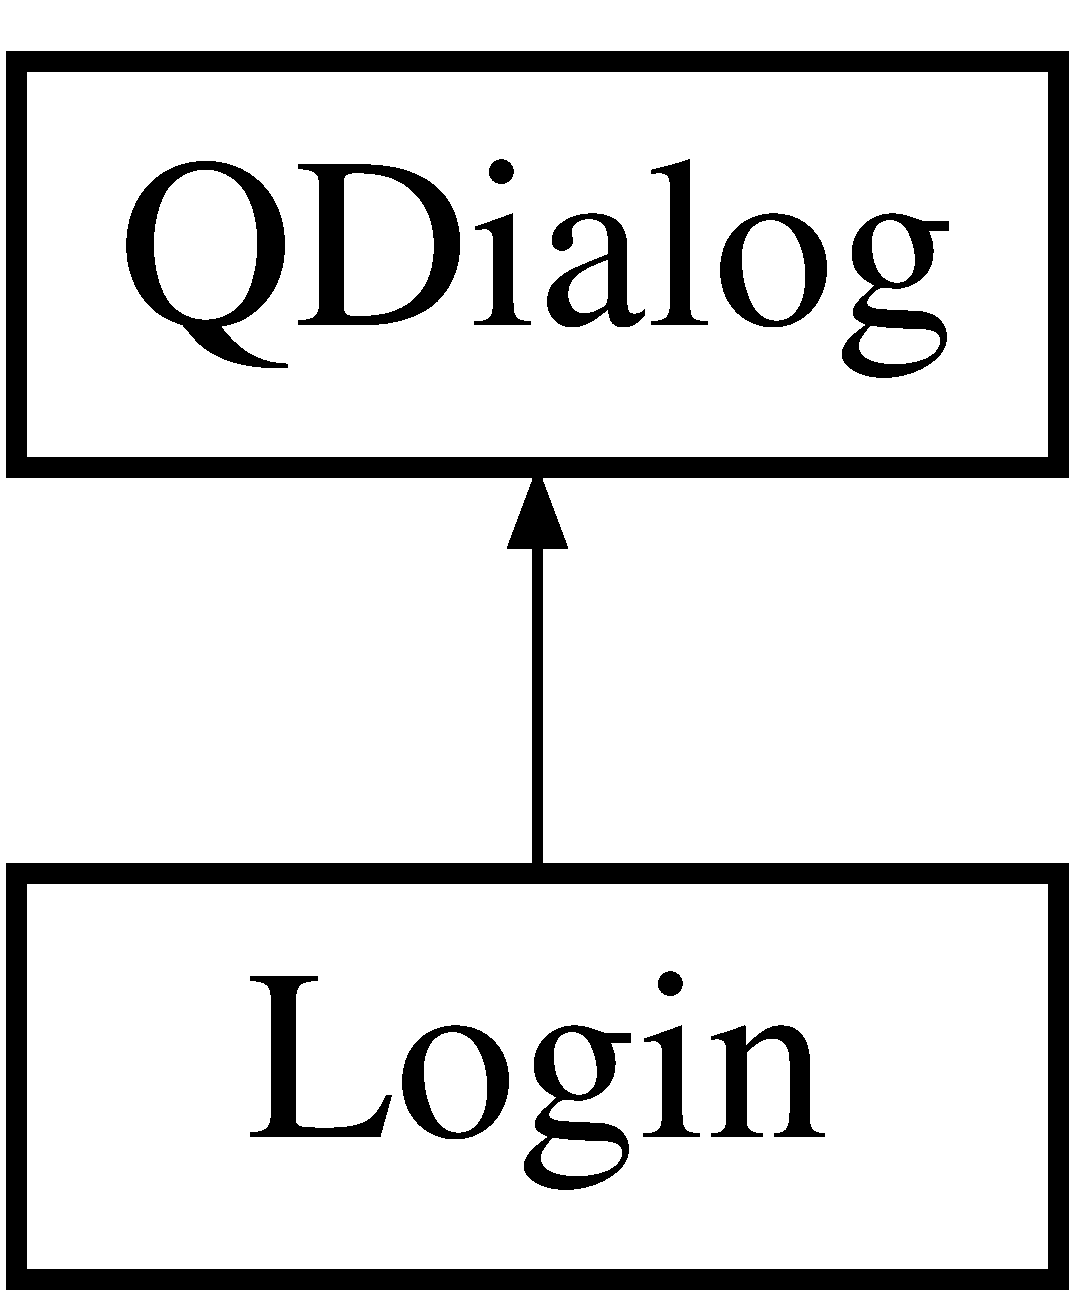
\includegraphics[height=2.000000cm]{class_login}
\end{center}
\end{figure}
\subsection*{Public Member Functions}
\begin{DoxyCompactItemize}
\item 
\mbox{\Hypertarget{class_login_a021ebcfd29b2a30e3f5c5bbb36589381}\label{class_login_a021ebcfd29b2a30e3f5c5bbb36589381}} 
{\bfseries Login} (Q\+Widget $\ast$parent=0)
\item 
bool \mbox{\hyperlink{class_login_ab6e2f801e7106b79425ae7c84bc8cd09}{autorisation}} ()
\begin{DoxyCompactList}\small\item\em autorisation \end{DoxyCompactList}\item 
\mbox{\Hypertarget{class_login_a6e5865295833745434c41e363fef3861}\label{class_login_a6e5865295833745434c41e363fef3861}} 
void \mbox{\hyperlink{class_login_a6e5865295833745434c41e363fef3861}{lire\+Fichier}} ()
\begin{DoxyCompactList}\small\item\em lire\+Fichier \end{DoxyCompactList}\end{DoxyCompactItemize}
\subsection*{Public Attributes}
\begin{DoxyCompactItemize}
\item 
\mbox{\Hypertarget{class_login_af691b5ea63279c19dc46d172ddd302a6}\label{class_login_af691b5ea63279c19dc46d172ddd302a6}} 
\mbox{\hyperlink{class_utilisateur}{Utilisateur}} \mbox{\hyperlink{class_login_af691b5ea63279c19dc46d172ddd302a6}{user}}
\begin{DoxyCompactList}\small\item\em user \end{DoxyCompactList}\end{DoxyCompactItemize}
\subsection*{Private Member Functions}
\begin{DoxyCompactItemize}
\item 
\mbox{\Hypertarget{class_login_a27cf76c5ec316c5ffe6df19817c578f6}\label{class_login_a27cf76c5ec316c5ffe6df19817c578f6}} 
void \mbox{\hyperlink{class_login_a27cf76c5ec316c5ffe6df19817c578f6}{enregistrement\+Login}} ()
\begin{DoxyCompactList}\small\item\em enregistrement\+Login \end{DoxyCompactList}\end{DoxyCompactItemize}
\subsection*{Private Attributes}
\begin{DoxyCompactItemize}
\item 
\mbox{\Hypertarget{class_login_a55fa3b19085f864462451d3dd9efd2e1}\label{class_login_a55fa3b19085f864462451d3dd9efd2e1}} 
Ui\+::\+Login $\ast$ {\bfseries ui}
\item 
\mbox{\Hypertarget{class_login_a1966b62cfe44e948028a67e615197c63}\label{class_login_a1966b62cfe44e948028a67e615197c63}} 
\mbox{\hyperlink{class_database}{Database}} \mbox{\hyperlink{class_login_a1966b62cfe44e948028a67e615197c63}{bdd}}
\begin{DoxyCompactList}\small\item\em bdd \end{DoxyCompactList}\end{DoxyCompactItemize}


\subsection{Detailed Description}
Classe \mbox{\hyperlink{class_login}{Login}} qui hérite de Q\+Dialog permet de gerer la fenetre login. 

\subsection{Member Function Documentation}
\mbox{\Hypertarget{class_login_ab6e2f801e7106b79425ae7c84bc8cd09}\label{class_login_ab6e2f801e7106b79425ae7c84bc8cd09}} 
\index{Login@{Login}!autorisation@{autorisation}}
\index{autorisation@{autorisation}!Login@{Login}}
\subsubsection{\texorpdfstring{autorisation()}{autorisation()}}
{\footnotesize\ttfamily bool Login\+::autorisation (\begin{DoxyParamCaption}{ }\end{DoxyParamCaption})}



autorisation 

\begin{DoxyReturn}{Returns}

\end{DoxyReturn}


The documentation for this class was generated from the following files\+:\begin{DoxyCompactItemize}
\item 
C\+:/\+Users/adai01/\+Desktop/\+Ware\+House\+Manager/\mbox{\hyperlink{login_8h}{login.\+h}}\item 
C\+:/\+Users/adai01/\+Desktop/\+Ware\+House\+Manager/login.\+cpp\end{DoxyCompactItemize}

\hypertarget{class_main_window}{}\section{Main\+Window Class Reference}
\label{class_main_window}\index{Main\+Window@{Main\+Window}}
Inheritance diagram for Main\+Window\+:\begin{figure}[H]
\begin{center}
\leavevmode
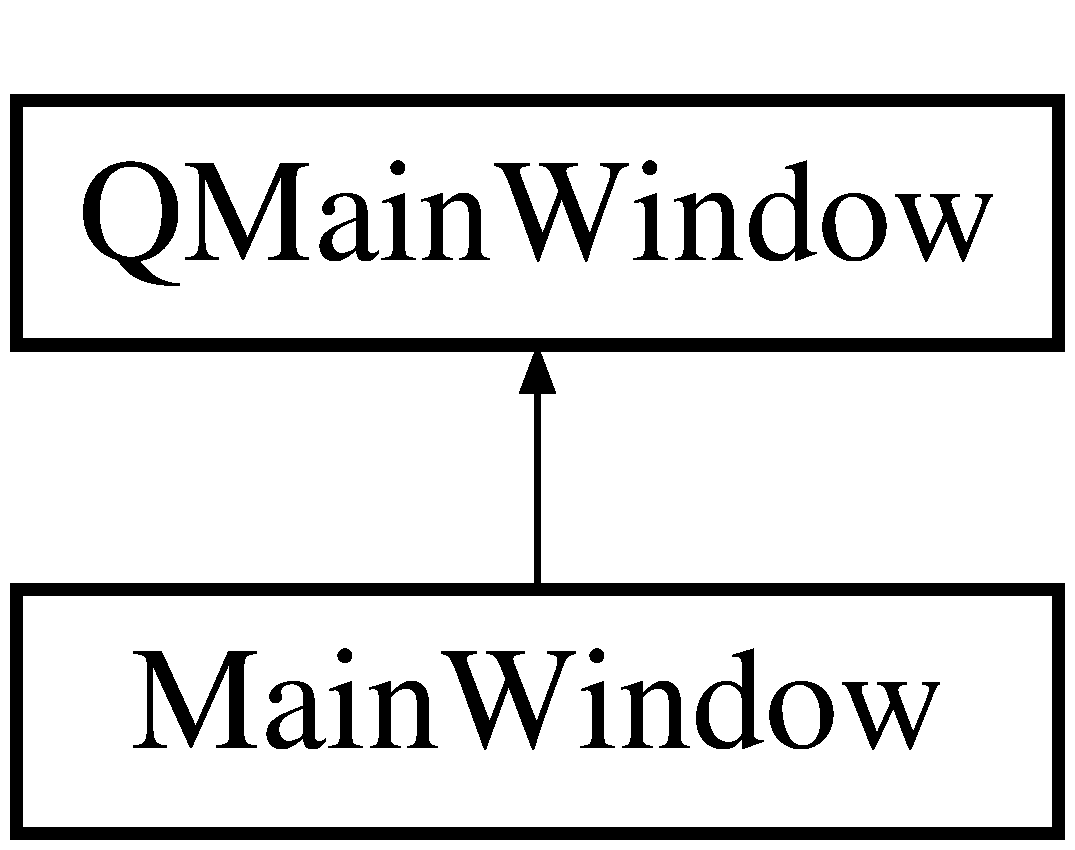
\includegraphics[height=2.000000cm]{class_main_window}
\end{center}
\end{figure}
\subsection*{Public Types}
\begin{DoxyCompactItemize}
\item 
\mbox{\Hypertarget{class_main_window_aa16f311e2d64ddecefd3eb2e17cdf800}\label{class_main_window_aa16f311e2d64ddecefd3eb2e17cdf800}} 
enum {\bfseries droits} \{ {\bfseries L\+O\+G\+I\+S\+T\+I\+C\+I\+EN} = 1, 
{\bfseries A\+D\+M\+I\+N\+I\+S\+T\+R\+A\+T\+E\+UR} = 2
 \}
\end{DoxyCompactItemize}
\subsection*{Public Slots}
\begin{DoxyCompactItemize}
\item 
\mbox{\Hypertarget{class_main_window_a94d1ec5b18a39e53c1700f907fb1f08e}\label{class_main_window_a94d1ec5b18a39e53c1700f907fb1f08e}} 
int {\bfseries on\+\_\+action\+Se\+\_\+deconnecter\+\_\+triggered} ()
\end{DoxyCompactItemize}
\subsection*{Public Member Functions}
\begin{DoxyCompactItemize}
\item 
\mbox{\Hypertarget{class_main_window_a8b244be8b7b7db1b08de2a2acb9409db}\label{class_main_window_a8b244be8b7b7db1b08de2a2acb9409db}} 
{\bfseries Main\+Window} (Q\+Widget $\ast$parent=0)
\item 
\mbox{\Hypertarget{class_main_window_ac600bafb6e03043944197a8eb6cf3cdb}\label{class_main_window_ac600bafb6e03043944197a8eb6cf3cdb}} 
void {\bfseries affiche\+Utilisateur} ()
\end{DoxyCompactItemize}
\subsection*{Public Attributes}
\begin{DoxyCompactItemize}
\item 
\mbox{\Hypertarget{class_main_window_a6d37265ebccf5d8891e033be9348133e}\label{class_main_window_a6d37265ebccf5d8891e033be9348133e}} 
\mbox{\hyperlink{class_utilisateur}{Utilisateur}} {\bfseries user}
\end{DoxyCompactItemize}


The documentation for this class was generated from the following files\+:\begin{DoxyCompactItemize}
\item 
mainwindow.\+h\item 
mainwindow.\+cpp\end{DoxyCompactItemize}

\hypertarget{class_utilisateur}{}\section{Utilisateur Class Reference}
\label{class_utilisateur}\index{Utilisateur@{Utilisateur}}


Classe \mbox{\hyperlink{class_utilisateur}{Utilisateur}} permettant de gerer les utilisateurs.  




{\ttfamily \#include $<$utilisateur.\+h$>$}

\subsection*{Public Member Functions}
\begin{DoxyCompactItemize}
\item 
\mbox{\Hypertarget{class_utilisateur_ae76433a6d353c5f5ad0c6a6af64022ad}\label{class_utilisateur_ae76433a6d353c5f5ad0c6a6af64022ad}} 
\mbox{\hyperlink{class_utilisateur_ae76433a6d353c5f5ad0c6a6af64022ad}{Utilisateur}} ()
\begin{DoxyCompactList}\small\item\em \mbox{\hyperlink{class_utilisateur}{Utilisateur}}. \end{DoxyCompactList}\item 
\mbox{\hyperlink{class_utilisateur_a9c279c4e14b76e43412e1480f3cfa07e}{Utilisateur}} (Q\+String \mbox{\hyperlink{class_utilisateur_abb16ed370d845def5c476b79ea415dba}{login}}, Q\+String \mbox{\hyperlink{class_utilisateur_a4f6a17d0fb5c231bcb414396236a056f}{mot\+De\+Passe}})
\begin{DoxyCompactList}\small\item\em \mbox{\hyperlink{class_utilisateur}{Utilisateur}}. \end{DoxyCompactList}\item 
\mbox{\hyperlink{class_utilisateur_a14ac7e9bd12689670dc386393f86045f}{Utilisateur}} (Q\+String \mbox{\hyperlink{class_utilisateur_abb16ed370d845def5c476b79ea415dba}{login}}, Q\+String \mbox{\hyperlink{class_utilisateur_a4f6a17d0fb5c231bcb414396236a056f}{mot\+De\+Passe}}, int \mbox{\hyperlink{class_utilisateur_ac4f7dfce4243768a6eabfbb57b883cdf}{droit}})
\begin{DoxyCompactList}\small\item\em \mbox{\hyperlink{class_utilisateur}{Utilisateur}}. \end{DoxyCompactList}\item 
Q\+String \mbox{\hyperlink{class_utilisateur_a3b830246e73edd798e0945e3b9904b93}{Get\+Login}} ()
\begin{DoxyCompactList}\small\item\em Get\+Login. \end{DoxyCompactList}\item 
Q\+String \mbox{\hyperlink{class_utilisateur_ad558f2e85090c4660e97e6de6f8d1567}{Get\+Mot\+De\+Passe}} ()
\begin{DoxyCompactList}\small\item\em Get\+Mot\+De\+Passe. \end{DoxyCompactList}\item 
int \mbox{\hyperlink{class_utilisateur_aa5e86f36e1b94dc3cce6393205c0a8cf}{Get\+Droit}} ()
\begin{DoxyCompactList}\small\item\em Get\+Droit. \end{DoxyCompactList}\item 
int \mbox{\hyperlink{class_utilisateur_a6cb20ba5bcbb83792e31f8a913178534}{Get\+Id}} ()
\begin{DoxyCompactList}\small\item\em Get\+Id. \end{DoxyCompactList}\item 
void \mbox{\hyperlink{class_utilisateur_a0bf37c85322764c3b094acd66aacec64}{Set\+Login}} (Q\+String \mbox{\hyperlink{class_utilisateur_abb16ed370d845def5c476b79ea415dba}{login}})
\begin{DoxyCompactList}\small\item\em Set\+Login. \end{DoxyCompactList}\item 
void \mbox{\hyperlink{class_utilisateur_a64504a89dd26ab7529305ea8d98460e5}{Set\+Mot\+De\+Passe}} (Q\+String \mbox{\hyperlink{class_utilisateur_a4f6a17d0fb5c231bcb414396236a056f}{mot\+De\+Passe}})
\begin{DoxyCompactList}\small\item\em Set\+Mot\+De\+Passe. \end{DoxyCompactList}\item 
void \mbox{\hyperlink{class_utilisateur_ab1d22e4a620262b9ea352b53872d855c}{Set\+Droit}} (int \mbox{\hyperlink{class_utilisateur_ac4f7dfce4243768a6eabfbb57b883cdf}{droit}})
\begin{DoxyCompactList}\small\item\em Set\+Droit. \end{DoxyCompactList}\item 
void \mbox{\hyperlink{class_utilisateur_a583802b49a289114a47911a4ac98158d}{Set\+Id}} (int \mbox{\hyperlink{class_utilisateur_a600c54bc097070179b64008dd98bdebb}{id}})
\begin{DoxyCompactList}\small\item\em Set\+Id. \end{DoxyCompactList}\end{DoxyCompactItemize}
\subsection*{Private Attributes}
\begin{DoxyCompactItemize}
\item 
\mbox{\Hypertarget{class_utilisateur_ac4f7dfce4243768a6eabfbb57b883cdf}\label{class_utilisateur_ac4f7dfce4243768a6eabfbb57b883cdf}} 
int \mbox{\hyperlink{class_utilisateur_ac4f7dfce4243768a6eabfbb57b883cdf}{droit}}
\begin{DoxyCompactList}\small\item\em droit \end{DoxyCompactList}\item 
\mbox{\Hypertarget{class_utilisateur_abb16ed370d845def5c476b79ea415dba}\label{class_utilisateur_abb16ed370d845def5c476b79ea415dba}} 
Q\+String \mbox{\hyperlink{class_utilisateur_abb16ed370d845def5c476b79ea415dba}{login}}
\begin{DoxyCompactList}\small\item\em login \end{DoxyCompactList}\item 
\mbox{\Hypertarget{class_utilisateur_a4f6a17d0fb5c231bcb414396236a056f}\label{class_utilisateur_a4f6a17d0fb5c231bcb414396236a056f}} 
Q\+String \mbox{\hyperlink{class_utilisateur_a4f6a17d0fb5c231bcb414396236a056f}{mot\+De\+Passe}}
\begin{DoxyCompactList}\small\item\em mot\+De\+Passe \end{DoxyCompactList}\item 
\mbox{\Hypertarget{class_utilisateur_a600c54bc097070179b64008dd98bdebb}\label{class_utilisateur_a600c54bc097070179b64008dd98bdebb}} 
int \mbox{\hyperlink{class_utilisateur_a600c54bc097070179b64008dd98bdebb}{id}}
\begin{DoxyCompactList}\small\item\em id \end{DoxyCompactList}\end{DoxyCompactItemize}


\subsection{Detailed Description}
Classe \mbox{\hyperlink{class_utilisateur}{Utilisateur}} permettant de gerer les utilisateurs. 

\subsection{Constructor \& Destructor Documentation}
\mbox{\Hypertarget{class_utilisateur_a9c279c4e14b76e43412e1480f3cfa07e}\label{class_utilisateur_a9c279c4e14b76e43412e1480f3cfa07e}} 
\index{Utilisateur@{Utilisateur}!Utilisateur@{Utilisateur}}
\index{Utilisateur@{Utilisateur}!Utilisateur@{Utilisateur}}
\subsubsection{\texorpdfstring{Utilisateur()}{Utilisateur()}\hspace{0.1cm}{\footnotesize\ttfamily [1/2]}}
{\footnotesize\ttfamily Utilisateur\+::\+Utilisateur (\begin{DoxyParamCaption}\item[{Q\+String}]{login,  }\item[{Q\+String}]{mot\+De\+Passe }\end{DoxyParamCaption})}



\mbox{\hyperlink{class_utilisateur}{Utilisateur}}. 


\begin{DoxyParams}{Parameters}
{\em login} & \\
\hline
{\em mot\+De\+Passe} & \\
\hline
\end{DoxyParams}
\mbox{\Hypertarget{class_utilisateur_a14ac7e9bd12689670dc386393f86045f}\label{class_utilisateur_a14ac7e9bd12689670dc386393f86045f}} 
\index{Utilisateur@{Utilisateur}!Utilisateur@{Utilisateur}}
\index{Utilisateur@{Utilisateur}!Utilisateur@{Utilisateur}}
\subsubsection{\texorpdfstring{Utilisateur()}{Utilisateur()}\hspace{0.1cm}{\footnotesize\ttfamily [2/2]}}
{\footnotesize\ttfamily Utilisateur\+::\+Utilisateur (\begin{DoxyParamCaption}\item[{Q\+String}]{login,  }\item[{Q\+String}]{mot\+De\+Passe,  }\item[{int}]{droit }\end{DoxyParamCaption})}



\mbox{\hyperlink{class_utilisateur}{Utilisateur}}. 


\begin{DoxyParams}{Parameters}
{\em login} & \\
\hline
{\em mot\+De\+Passe} & \\
\hline
{\em droit} & \\
\hline
\end{DoxyParams}


\subsection{Member Function Documentation}
\mbox{\Hypertarget{class_utilisateur_aa5e86f36e1b94dc3cce6393205c0a8cf}\label{class_utilisateur_aa5e86f36e1b94dc3cce6393205c0a8cf}} 
\index{Utilisateur@{Utilisateur}!Get\+Droit@{Get\+Droit}}
\index{Get\+Droit@{Get\+Droit}!Utilisateur@{Utilisateur}}
\subsubsection{\texorpdfstring{Get\+Droit()}{GetDroit()}}
{\footnotesize\ttfamily int Utilisateur\+::\+Get\+Droit (\begin{DoxyParamCaption}{ }\end{DoxyParamCaption})}



Get\+Droit. 

\begin{DoxyReturn}{Returns}

\end{DoxyReturn}
\mbox{\Hypertarget{class_utilisateur_a6cb20ba5bcbb83792e31f8a913178534}\label{class_utilisateur_a6cb20ba5bcbb83792e31f8a913178534}} 
\index{Utilisateur@{Utilisateur}!Get\+Id@{Get\+Id}}
\index{Get\+Id@{Get\+Id}!Utilisateur@{Utilisateur}}
\subsubsection{\texorpdfstring{Get\+Id()}{GetId()}}
{\footnotesize\ttfamily int Utilisateur\+::\+Get\+Id (\begin{DoxyParamCaption}{ }\end{DoxyParamCaption})}



Get\+Id. 

\begin{DoxyReturn}{Returns}

\end{DoxyReturn}
\mbox{\Hypertarget{class_utilisateur_a3b830246e73edd798e0945e3b9904b93}\label{class_utilisateur_a3b830246e73edd798e0945e3b9904b93}} 
\index{Utilisateur@{Utilisateur}!Get\+Login@{Get\+Login}}
\index{Get\+Login@{Get\+Login}!Utilisateur@{Utilisateur}}
\subsubsection{\texorpdfstring{Get\+Login()}{GetLogin()}}
{\footnotesize\ttfamily Q\+String Utilisateur\+::\+Get\+Login (\begin{DoxyParamCaption}{ }\end{DoxyParamCaption})}



Get\+Login. 

\begin{DoxyReturn}{Returns}

\end{DoxyReturn}
\mbox{\Hypertarget{class_utilisateur_ad558f2e85090c4660e97e6de6f8d1567}\label{class_utilisateur_ad558f2e85090c4660e97e6de6f8d1567}} 
\index{Utilisateur@{Utilisateur}!Get\+Mot\+De\+Passe@{Get\+Mot\+De\+Passe}}
\index{Get\+Mot\+De\+Passe@{Get\+Mot\+De\+Passe}!Utilisateur@{Utilisateur}}
\subsubsection{\texorpdfstring{Get\+Mot\+De\+Passe()}{GetMotDePasse()}}
{\footnotesize\ttfamily Q\+String Utilisateur\+::\+Get\+Mot\+De\+Passe (\begin{DoxyParamCaption}{ }\end{DoxyParamCaption})}



Get\+Mot\+De\+Passe. 

\begin{DoxyReturn}{Returns}

\end{DoxyReturn}
\mbox{\Hypertarget{class_utilisateur_ab1d22e4a620262b9ea352b53872d855c}\label{class_utilisateur_ab1d22e4a620262b9ea352b53872d855c}} 
\index{Utilisateur@{Utilisateur}!Set\+Droit@{Set\+Droit}}
\index{Set\+Droit@{Set\+Droit}!Utilisateur@{Utilisateur}}
\subsubsection{\texorpdfstring{Set\+Droit()}{SetDroit()}}
{\footnotesize\ttfamily void Utilisateur\+::\+Set\+Droit (\begin{DoxyParamCaption}\item[{int}]{droit }\end{DoxyParamCaption})}



Set\+Droit. 


\begin{DoxyParams}{Parameters}
{\em droit} & \\
\hline
\end{DoxyParams}
\mbox{\Hypertarget{class_utilisateur_a583802b49a289114a47911a4ac98158d}\label{class_utilisateur_a583802b49a289114a47911a4ac98158d}} 
\index{Utilisateur@{Utilisateur}!Set\+Id@{Set\+Id}}
\index{Set\+Id@{Set\+Id}!Utilisateur@{Utilisateur}}
\subsubsection{\texorpdfstring{Set\+Id()}{SetId()}}
{\footnotesize\ttfamily void Utilisateur\+::\+Set\+Id (\begin{DoxyParamCaption}\item[{int}]{id }\end{DoxyParamCaption})}



Set\+Id. 


\begin{DoxyParams}{Parameters}
{\em id} & \\
\hline
\end{DoxyParams}
\mbox{\Hypertarget{class_utilisateur_a0bf37c85322764c3b094acd66aacec64}\label{class_utilisateur_a0bf37c85322764c3b094acd66aacec64}} 
\index{Utilisateur@{Utilisateur}!Set\+Login@{Set\+Login}}
\index{Set\+Login@{Set\+Login}!Utilisateur@{Utilisateur}}
\subsubsection{\texorpdfstring{Set\+Login()}{SetLogin()}}
{\footnotesize\ttfamily void Utilisateur\+::\+Set\+Login (\begin{DoxyParamCaption}\item[{Q\+String}]{login }\end{DoxyParamCaption})}



Set\+Login. 


\begin{DoxyParams}{Parameters}
{\em login} & \\
\hline
\end{DoxyParams}
\mbox{\Hypertarget{class_utilisateur_a64504a89dd26ab7529305ea8d98460e5}\label{class_utilisateur_a64504a89dd26ab7529305ea8d98460e5}} 
\index{Utilisateur@{Utilisateur}!Set\+Mot\+De\+Passe@{Set\+Mot\+De\+Passe}}
\index{Set\+Mot\+De\+Passe@{Set\+Mot\+De\+Passe}!Utilisateur@{Utilisateur}}
\subsubsection{\texorpdfstring{Set\+Mot\+De\+Passe()}{SetMotDePasse()}}
{\footnotesize\ttfamily void Utilisateur\+::\+Set\+Mot\+De\+Passe (\begin{DoxyParamCaption}\item[{Q\+String}]{mot\+De\+Passe }\end{DoxyParamCaption})}



Set\+Mot\+De\+Passe. 


\begin{DoxyParams}{Parameters}
{\em mot\+De\+Passe} & \\
\hline
\end{DoxyParams}


The documentation for this class was generated from the following files\+:\begin{DoxyCompactItemize}
\item 
C\+:/\+Users/adai01/\+Desktop/\+Ware\+House\+Manager/\mbox{\hyperlink{utilisateur_8h}{utilisateur.\+h}}\item 
C\+:/\+Users/adai01/\+Desktop/\+Ware\+House\+Manager/utilisateur.\+cpp\end{DoxyCompactItemize}

\chapter{File Documentation}
\hypertarget{article_8h}{}\section{C\+:/\+Users/adai01/\+Desktop/\+Ware\+House\+Manager/article.h File Reference}
\label{article_8h}\index{C\+:/\+Users/adai01/\+Desktop/\+Ware\+House\+Manager/article.\+h@{C\+:/\+Users/adai01/\+Desktop/\+Ware\+House\+Manager/article.\+h}}


Gestion des articles.  


{\ttfamily \#include $<$Q\+String$>$}\newline
\subsection*{Classes}
\begin{DoxyCompactItemize}
\item 
class \mbox{\hyperlink{class_article}{Article}}
\begin{DoxyCompactList}\small\item\em Classe \mbox{\hyperlink{class_article}{Article}} permettant de gerer les articles. \end{DoxyCompactList}\end{DoxyCompactItemize}


\subsection{Detailed Description}
Gestion des articles. 

\begin{DoxyAuthor}{Author}
Cédric B\+A\+N\+N\+E\+L\+I\+ER 
\end{DoxyAuthor}
\begin{DoxyVersion}{Version}
0.\+1b 
\end{DoxyVersion}

\hypertarget{database_8h}{}\section{C\+:/\+Users/adai01/\+Desktop/\+Ware\+House\+Manager/database.h File Reference}
\label{database_8h}\index{C\+:/\+Users/adai01/\+Desktop/\+Ware\+House\+Manager/database.\+h@{C\+:/\+Users/adai01/\+Desktop/\+Ware\+House\+Manager/database.\+h}}


Gestion de toutes les requetes S\+QL.  


{\ttfamily \#include $<$Q\+String$>$}\newline
{\ttfamily \#include $<$Qt\+Sql/\+Qt\+Sql$>$}\newline
{\ttfamily \#include \char`\"{}article.\+h\char`\"{}}\newline
{\ttfamily \#include \char`\"{}utilisateur.\+h\char`\"{}}\newline
{\ttfamily \#include \char`\"{}emballage.\+h\char`\"{}}\newline
{\ttfamily \#include \char`\"{}fournisseur.\+h\char`\"{}}\newline
{\ttfamily \#include \char`\"{}livraison.\+h\char`\"{}}\newline
\subsection*{Classes}
\begin{DoxyCompactItemize}
\item 
class \mbox{\hyperlink{class_database}{Database}}
\begin{DoxyCompactList}\small\item\em Classe \mbox{\hyperlink{class_database}{Database}} permettant de gerer les requetes S\+QL. Dans cette classe toutes les requetes sont présentes. \end{DoxyCompactList}\end{DoxyCompactItemize}


\subsection{Detailed Description}
Gestion de toutes les requetes S\+QL. 

\begin{DoxyAuthor}{Author}
Cédric B\+A\+N\+N\+E\+L\+I\+ER 
\end{DoxyAuthor}
\begin{DoxyVersion}{Version}
0.\+1b 
\end{DoxyVersion}

\hypertarget{emballage_8h}{}\section{C\+:/\+Users/adai01/\+Desktop/\+Ware\+House\+Manager/emballage.h File Reference}
\label{emballage_8h}\index{C\+:/\+Users/adai01/\+Desktop/\+Ware\+House\+Manager/emballage.\+h@{C\+:/\+Users/adai01/\+Desktop/\+Ware\+House\+Manager/emballage.\+h}}


Gestion des emballages.  


{\ttfamily \#include $<$Q\+String$>$}\newline
\subsection*{Classes}
\begin{DoxyCompactItemize}
\item 
class \mbox{\hyperlink{class_emballage}{Emballage}}
\begin{DoxyCompactList}\small\item\em Classe \mbox{\hyperlink{class_emballage}{Emballage}} permettant de gerer les emballages. \end{DoxyCompactList}\end{DoxyCompactItemize}


\subsection{Detailed Description}
Gestion des emballages. 

\begin{DoxyAuthor}{Author}
Cédric B\+A\+N\+N\+E\+L\+I\+ER 
\end{DoxyAuthor}
\begin{DoxyVersion}{Version}
0.\+1b 
\end{DoxyVersion}

\hypertarget{fournisseur_8h}{}\section{C\+:/\+Users/adai01/\+Desktop/\+Ware\+House\+Manager/fournisseur.h File Reference}
\label{fournisseur_8h}\index{C\+:/\+Users/adai01/\+Desktop/\+Ware\+House\+Manager/fournisseur.\+h@{C\+:/\+Users/adai01/\+Desktop/\+Ware\+House\+Manager/fournisseur.\+h}}


Gestion des fournisseurs.  


{\ttfamily \#include $<$Q\+String$>$}\newline
\subsection*{Classes}
\begin{DoxyCompactItemize}
\item 
class \mbox{\hyperlink{class_fournisseur}{Fournisseur}}
\begin{DoxyCompactList}\small\item\em Classe \mbox{\hyperlink{class_fournisseur}{Fournisseur}} permettant de gerer les fournisseurs. \end{DoxyCompactList}\end{DoxyCompactItemize}


\subsection{Detailed Description}
Gestion des fournisseurs. 

\begin{DoxyAuthor}{Author}
Cédric B\+A\+N\+N\+E\+L\+I\+ER 
\end{DoxyAuthor}
\begin{DoxyVersion}{Version}
0.\+1b 
\end{DoxyVersion}

\hypertarget{livraison_8h}{}\section{C\+:/\+Users/adai01/\+Desktop/\+Ware\+House\+Manager/livraison.h File Reference}
\label{livraison_8h}\index{C\+:/\+Users/adai01/\+Desktop/\+Ware\+House\+Manager/livraison.\+h@{C\+:/\+Users/adai01/\+Desktop/\+Ware\+House\+Manager/livraison.\+h}}


Gestion des livraisons.  


{\ttfamily \#include $<$Q\+String$>$}\newline
\subsection*{Classes}
\begin{DoxyCompactItemize}
\item 
class \mbox{\hyperlink{class_livraison}{Livraison}}
\begin{DoxyCompactList}\small\item\em Classe \mbox{\hyperlink{class_livraison}{Livraison}} permettant de gerer les livraisons. \end{DoxyCompactList}\end{DoxyCompactItemize}


\subsection{Detailed Description}
Gestion des livraisons. 

\begin{DoxyAuthor}{Author}
Cédric B\+A\+N\+N\+E\+L\+I\+ER 
\end{DoxyAuthor}
\begin{DoxyVersion}{Version}
0.\+1b 
\end{DoxyVersion}

\hypertarget{login_8h}{}\section{C\+:/\+Users/adai01/\+Desktop/\+Ware\+House\+Manager/login.h File Reference}
\label{login_8h}\index{C\+:/\+Users/adai01/\+Desktop/\+Ware\+House\+Manager/login.\+h@{C\+:/\+Users/adai01/\+Desktop/\+Ware\+House\+Manager/login.\+h}}


Gestion des logins.  


{\ttfamily \#include $<$Q\+Dialog$>$}\newline
{\ttfamily \#include \char`\"{}database.\+h\char`\"{}}\newline
{\ttfamily \#include \char`\"{}mainwindow.\+h\char`\"{}}\newline
{\ttfamily \#include \char`\"{}utilisateur.\+h\char`\"{}}\newline
\subsection*{Classes}
\begin{DoxyCompactItemize}
\item 
class \mbox{\hyperlink{class_login}{Login}}
\begin{DoxyCompactList}\small\item\em Classe \mbox{\hyperlink{class_login}{Login}} qui hérite de Q\+Dialog permet de gerer la fenetre login. \end{DoxyCompactList}\end{DoxyCompactItemize}


\subsection{Detailed Description}
Gestion des logins. 

\begin{DoxyAuthor}{Author}
Cédric B\+A\+N\+N\+E\+L\+I\+ER 
\end{DoxyAuthor}
\begin{DoxyVersion}{Version}
0.\+1b 
\end{DoxyVersion}

\hypertarget{mainwindow_8h}{}\section{C\+:/\+Users/adai01/\+Desktop/\+Ware\+House\+Manager/mainwindow.h File Reference}
\label{mainwindow_8h}\index{C\+:/\+Users/adai01/\+Desktop/\+Ware\+House\+Manager/mainwindow.\+h@{C\+:/\+Users/adai01/\+Desktop/\+Ware\+House\+Manager/mainwindow.\+h}}


fenetre principale de l\textquotesingle{}application  


{\ttfamily \#include $<$Q\+Main\+Window$>$}\newline
{\ttfamily \#include $<$Q\+Line\+Edit$>$}\newline
{\ttfamily \#include $<$Q\+Dialog$>$}\newline
{\ttfamily \#include $<$Q\+Dialog\+Button\+Box$>$}\newline
{\ttfamily \#include $<$Q\+Message\+Box$>$}\newline
{\ttfamily \#include $<$Q\+Label$>$}\newline
{\ttfamily \#include $<$Q\+Table\+View$>$}\newline
{\ttfamily \#include $<$Q\+Standard\+Item\+Model$>$}\newline
{\ttfamily \#include \char`\"{}utilisateur.\+h\char`\"{}}\newline
{\ttfamily \#include \char`\"{}database.\+h\char`\"{}}\newline
{\ttfamily \#include \char`\"{}login.\+h\char`\"{}}\newline
\subsection*{Classes}
\begin{DoxyCompactItemize}
\item 
class \mbox{\hyperlink{class_main_window}{Main\+Window}}
\begin{DoxyCompactList}\small\item\em Classe \mbox{\hyperlink{class_main_window}{Main\+Window}} qui herite de la Q\+Main\+Window. Fenêtre principale de l\textquotesingle{}application. \end{DoxyCompactList}\end{DoxyCompactItemize}


\subsection{Detailed Description}
fenetre principale de l\textquotesingle{}application 

\begin{DoxyAuthor}{Author}
Cédric B\+A\+N\+N\+E\+L\+I\+ER 
\end{DoxyAuthor}
\begin{DoxyVersion}{Version}
0.\+1b 
\end{DoxyVersion}

\hypertarget{utilisateur_8h}{}\section{C\+:/\+Users/adai01/\+Desktop/\+Ware\+House\+Manager/utilisateur.h File Reference}
\label{utilisateur_8h}\index{C\+:/\+Users/adai01/\+Desktop/\+Ware\+House\+Manager/utilisateur.\+h@{C\+:/\+Users/adai01/\+Desktop/\+Ware\+House\+Manager/utilisateur.\+h}}


Gestion des utilisateurs.  


{\ttfamily \#include $<$Q\+String$>$}\newline
\subsection*{Classes}
\begin{DoxyCompactItemize}
\item 
class \mbox{\hyperlink{class_utilisateur}{Utilisateur}}
\begin{DoxyCompactList}\small\item\em Classe \mbox{\hyperlink{class_utilisateur}{Utilisateur}} permettant de gerer les utilisateurs. \end{DoxyCompactList}\end{DoxyCompactItemize}


\subsection{Detailed Description}
Gestion des utilisateurs. 

\begin{DoxyAuthor}{Author}
Cédric B\+A\+N\+N\+E\+L\+I\+ER 
\end{DoxyAuthor}
\begin{DoxyVersion}{Version}
0.\+1b 
\end{DoxyVersion}

%--- End generated contents ---

% Index
\backmatter
\newpage
\phantomsection
\clearemptydoublepage
\addcontentsline{toc}{chapter}{Index}
\printindex

\end{document}
